\documentclass[12pt]{article}
\usepackage[margin=1.1in]{geometry}
\usepackage{amsmath,amssymb,amsthm}
\usepackage[round]{natbib}
\usepackage{setspace}
% JCGS submission build: flip to \jcgstrue for double spacing
\newif\ifjcgs
\jcgsfalse
\ifjcgs\doublespacing\fi
\usepackage{graphicx}
\usepackage{booktabs}
\usepackage{algorithm}
\usepackage{algpseudocode}
\usepackage[hidelinks]{hyperref}
\hypersetup{pdftitle={Scalable Share Calibration for Factor Multinomial Probit Models},
pdfauthor={Peter Cotton}}

\newtheorem{proposition}{Proposition}
\newtheorem{theorem}{Theorem}
\theoremstyle{remark}
\newtheorem{remark}{Remark}

\newcommand{\E}{\mathbb{E}}
\newcommand{\Prob}{\mathbb{P}}

\title{Scalable Share Calibration for\\ Factor Multinomial Probit Models}
\author{Peter Cotton\thanks{peter.cotton@microprediction.com. Every
number in this paper is produced by a committed, seeded script; see
Reproducibility and Supplementary Materials.}}
\date{August 2026}

\begin{document}
\maketitle

\begin{abstract}
We give an algorithm that inverts observed shares to utilities in
multinomial probit models with many alternatives, when the covariance
is low-rank-plus-diagonal and supplied. Conditioning on the factors
makes the alternatives independent, so one shared survival field prices
all $N$ alternatives in a single pass over $Q$ factor nodes and $L$
grid points, at $O(QNL)$ cost. The same field yields resampling-free
Jacobian--vector products, and share inversion at $N = 1000$ takes
three seconds in the compiled implementation at rank two. Ten thousand
alternatives stay under a minute. In convergence comparisons, the
computed shares carry log-share errors of a few parts in a hundred
thousand, hundred-to-one shares included. The established
high-precision evaluators price one orthant at a time. The nearest
factor-aware competitor computes the same share vector roughly
$140\times$ slower at matched accuracy at $N = 1000$, and the gap
widens linearly in $N$.
\end{abstract}

\noindent\textbf{Keywords:} multinomial probit; discrete choice;
numerical quadrature; Jacobian--vector product; share inversion; factor
model

\section{Introduction}

Probit models find their most traditional application in microeconomics, choice, and contest theory. 
Thurstone's comparative judgment, the ordered and binary probits of applied
microeconometrics, and the Lazear--Rosen tournament
\citep{lazear1981} are all the same
Gaussian latent-performance model. Machine learning runs on the same
family: a softmax output layer is its Luce--Gumbel member
\citep{luce1959,yellott1977}, and
Thurstone--Mosteller pairwise comparison \citep{mosteller1951}, the
probit member, underlies
rating systems and preference learning.

The same engine was canonized independently, under different names,
across the quantitative sciences. Bioassay named the probit and made
Gaussian tolerances the dose--response standard
\citep{bliss1934,finney1947}. Quantitative genetics reports the
heritability of binary traits on the liability scale, a thresholded
latent Gaussian \citep{dempster1950,falconer1965}. Item response theory
began with the normal-ogive curve and adopted the logistic only as a
computational stand-in \citep{lord1952}.

Signal detection's $d'$ is a
double probit \citep{green1966}. The Basel capital formula that
regulates the world's banks is a conditional probit with one common
factor \citep{vasicek2002,gordy2003}, which is to say a rank-one factor
model of exactly the form used here. Machine learning made probit its
tractable Bayesian classifier \citep{albertchib1993} and ships a
Thurstonian race as its skill-rating engine \citep{herbrich2006}.
Wherever performance is latent and Gaussian, the same object appears.

With unrestricted alternative intercepts, a single interior share
vector\footnote{We call the choice probabilities $p_i$ \emph{shares} throughout. The racing origin \citep{cotton2021} called them \emph{state prices}, borrowing prediction-market and finance usage. In the probit choice setting \emph{shares}, as in market shares, is the more natural term. \emph{Probability} would also be imprecise on the discrete lattice used later, where ties have positive probability and a dead heat splits the payout. The lattice objects really are state prices.} cannot distinguish full-support random-utility models, because
each can be inverted to match it. However, when logit, probit, or other models are calibrated to observed shares, the recovered utilities can serve as inputs to questions the data do not answer
directly: elasticities, welfare, pricing, the effect of adding or
removing an alternative, and combinatorial probabilities. It is at this point that they make different, falsifiable predictions. 

Judged by popularity, the workhorse of econometrics
remains the logit family: multinomial logit,
nested logit, and above all random-coefficients logit in the Berry--Levinsohn--Pakes (BLP) tradition
\citep{berry1995,train2009,conlon2020}. A major reason for logit's dominance is brutally practical. Logit
models can be computed.

Choice modeling did not start there. It started with Thurstone's 1927 model
\citep{thurstone1927} of jointly Gaussian utilities with unrestricted
correlation, brought into econometrics as the conditional (multinomial)
probit model by \citet{hausman1978} and known since as MNP. The same
object has re-emerged in machine learning: conditional on an input,
heteroskedastic image classifiers place exactly this
low-rank-plus-diagonal Gaussian race on their final layer and take the
argmax, approximating the winner probabilities by Monte Carlo over a
softmax relaxation \citep{collier2021}.

Probit probabilities are $(N-1)$-dimensional Gaussian integrals with,
generically, no closed form. A well-cited approach is the Geweke--Hajivassiliou--Keane
(GHK) simulator \citep{geweke1994,hajivassiliou1998,train2009}, the
econometric branch of the Genz separation-of-variables family
\citep{genz1992} whose randomized quasi-Monte Carlo (RQMC) form
(Genz--Bretz) is the default in
computational statistics.  This method treats
the probability that alternative $i$ beats the rest as an orthant
probability of the difference utilities, and estimates it by sampling
truncated normals sequentially along a Cholesky factor.

GHK is elegant, but it evaluates each winner event as a separate
orthant probability. With ordinary Monte Carlo its stochastic error is
$O(R^{-1/2})$ in the number of draws. RQMC often improves the empirical
rate, but the method remains stochastic, resolved by draw count, and it
still prices one orthant per alternative. The structural issue is that
none of these formulations exploit the product shared across the $N$
winner events.

The field kept the
computable models and gave up the model it started from. The concession
is not free. Logit-family substitution is structurally
restricted. One measure of the cost comes from an oracle factor-probit
benchmark with every marginal variance held at one
(Section~\ref{sec:boundary}). We generate a Gaussian factor race,
calibrate both models to identical menu shares, delete an alternative,
and ask where its demand goes. Among deletions of the largest
alternatives, plain logit misallocates a median 25\% of the released
demand, against 1\% for the correctly specified factor model
(experiment 29).\footnote{Experiment numbers index committed, seeded
scripts in the repository; see the Reproducibility section.} A companion factorial with a deliberately misspecified
truth tells a similar story.

We take the Gaussian race as the natural starting point, an argument
developed in Section~\ref{sec:applications}, and the deletion experiments below measure
its consequences under known synthetic truths. Any empirical argument for one race over the other on
real data is deferred to a companion survey \citep{cottonsurvey}. The
sustained literature on probit computation is evidence in itself that
the model is worth computing.

This paper's sole point is that probit's computational barrier is not real for an important
class of covariance structures, the low-rank-plus-diagonal factor model
\[
\Sigma = VV^\top + \mathrm{diag}(D).
\]
These are races where each
performance is idiosyncratic but also influenced by a small number of
factors common to all runners. The goal is \emph{calibration}: given
observed shares and a fixed, known factor structure $(V, D)$, recover the
utilities at which the probit model reproduces them.\footnote{In racing
parlance, we are recovering the relative ability of horses from the
bookmaker odds, even when some horses are known to be correlated with
others. The original transform \citep{cotton2021} assumed independent
performances.} 

We solve this fixed factor-probit share calibration problem at $N = 1000$ alternatives
in three seconds at rank two with the compiled implementation. The computation is the probit analogue of a far more popular logit inversion. For example, 
demand estimation runs on the logit side every day \citep{berry1995,conlon2020}.\footnote{Estimating $(V, D)$ is the outer problem. It is discussed in
Section~\ref{sec:discussion} but not claimed here.} 

The share map is also globally identified and onto the simplex interior
(Proposition~\ref{thm:inv}: shares determine utilities uniquely up to
location). 

Three ingredients make this possible: 

\begin{enumerate}
\item \emph{A fast forward map} (utilities $\to$ shares): all $N$
probabilities at once in $O(QNL)$ for $Q$ factor nodes and $L$ lattice
points. Calibration needs many forward evaluations; this is what makes
them affordable.
\item \emph{Resampling-free derivatives}: Jacobian--vector products in
$O(QNL)$. The Jacobian is a weighted graph
Laplacian, so reduced systems are symmetric positive definite. This supports
implicit differentiation and Newton--Krylov solvers. The calibration
reported below uses a cheaper damped Jacobi iteration.
\item \emph{A single shared construction}: conditionally on the $k$
factors (the rank) the alternatives are independent, and a lattice survival-product
identity computes every alternative's integral from one \emph{shared
survival field}, built once and reused for shares, slopes, and all $N$
single-removal counterfactuals.
\end{enumerate}

This one-pass identity comes from a mildly obscure but fitting literature: inferring ability
from win probabilities in multi-entrant races \citep{cotton2021}. That
work already emphasized very large fields and applications beyond the
track, digital commerce among them. The central trick this paper
leans heavily on was described there as a multiplicity calculus: a characterization of tie density 
on a lattice and a set of algebraic operations for combining races and removing a runner. That is
perhaps why it has not been assembled for probit before, where the focus has been on more classical methods
for numerical computation. No single ingredient here is new. The contribution is the
combination: factor conditioning, all-$N$ computation, derivatives,
inversion, and implementation at $N = 10^4$.

\section{The algorithm}\label{sec:algorithm}

We assume throughout a known factor structure. That structure is, as
it happens, the one with which correlated utilities entered
econometrics. \citet{hausman1978} induced correlation
through random taste coefficients, giving a covariance that is exactly
low-rank plus diagonal with observed attributes as loadings. Freeing the
loadings is the factor-analytic MNP that \citet{mcfadden1984} proposed
precisely to reduce the dimension of the integral. 

\paragraph{Model.} Throughout,
\begin{equation}
U_i \;=\; \mu_i + v_i^\top f + \sqrt{D_i}\,\varepsilon_i,
\qquad f \sim N(0, I_k), \quad \varepsilon_i \sim N(0,1) \text{ i.i.d.},
\quad D_i > 0,
\label{eq:model}
\end{equation}
i.e.\ $\Sigma = VV^\top + \mathrm{diag}(D)$. The chosen alternative is the
argmax of $U$. The pair $(V, D)$ is supplied and held fixed.
Calibration solves for $\mu$ alone.

Conditional on the factors, the alternatives are independent, and the
algorithm is built entirely on that fact. Write $g_i(\cdot \mid f)$ and
$F_i(\cdot \mid f)$ for the conditional density and cumulative distribution function (CDF) of $U_i$ given
$f$. Alternative $i$ wins when it beats every rival, so
\begin{equation}
p_i \;=\; \E_f\!\left[\;\int g_i(x \mid f)
\prod_{j \neq i} F_j(x \mid f)\, dx \right],
\qquad \sum_i p_i = 1,
\label{eq:forward}
\end{equation}
the shares summing to one because ties are null for continuous laws.
The $N$ products need not be formed
separately. Compute $\log F_{\mathrm{field}} = \sum_j \log F_j$ once.
Each product over $j \ne i$ is then recovered by subtracting the own
term.

The forward pass proceeds as follows. Lay down one common
grid of $L$ points, wide enough to contain every runner's distribution
at every retained factor node. We call this interval the
\emph{envelope}. At each factor node $f_q$, shift each
runner's location by $v_i^\top f_q$ and evaluate each runner's
log-survival curve on the grid. This is the log-probability that runner
$i$ has not yet finished by position $x$. Sum these $N$ curves to obtain the
\emph{shared survival field}, the log-probability that nobody has
finished by $x$. To price runner $i$, subtract its own log-survival
back out of the field, multiply by its density, and integrate along the
grid. This is the probability that $i$ finishes first at this factor
node, with everyone else behind.\footnote{This divide-one-out step is
the ``removing a runner'' operation of the multiplicity calculus in
\citet{cotton2021}, applied here once per alternative against a field
built only once.} Average over factor nodes with the
quadrature weights, and normalize. Everything is done in the log domain
so that deep-tail survivals never underflow. Algorithm~\ref{alg:forward}
states this precisely.

A lattice of a few hundred points and a pruned product Gauss--Hermite
rule suffice in practice. The exact resolution settings, and the
evidence that they are converged, are collected with the numerical
results in Section~\ref{sec:benchmark}.

Algorithm~\ref{alg:forward} works in reflected \emph{min-wins}
coordinates $a = -\mu$, a race won by the smallest value, while the
theory is stated in the natural \emph{max-wins} coordinates $\mu$; the reflection
keeps the loadings' sign. It is valid
because the Gaussian law is unchanged under $(f, \varepsilon) \mapsto
(-f, -\varepsilon)$.

\begin{algorithm}[H]
\caption{All-share forward pass (min-wins; reflected from argmax by $a = -\mu$)}
\label{alg:forward}
\begin{algorithmic}[1]
\Require abilities $a$, loadings $V$, idiosyncratic variances $D$, factor
nodes $\{f_q, w_q\}_{q=1}^{Q}$, lattice size $L$
\State $m_{iq} \gets a_i + v_i^\top f_q$ for all $i, q$
\State $[x_1, x_L] \gets [\min_{i,q} m_{iq} - 8\max_i \sqrt{D_i},\;
\max_{i,q} m_{iq} + 8\max_i \sqrt{D_i}]$, uniform spacing $\Delta x$
\For{$q = 1, \dots, Q$}
  \State $\log S_i(x_\ell) \gets \log\Phi\big({-(x_\ell -
  m_{iq})}/{\sqrt{D_i}}\big)$ for all $i, \ell$
  \Comment{never $1 - \Phi$}
  \State $\log S_{\mathrm{field}}(x_\ell) \gets \sum_j \log
  S_j(x_\ell)$
  \Comment{one shared field}
  \State $\tilde p_i \mathrel{+}= w_q \sum_\ell g_i(x_\ell)\,
  \exp\{\log S_{\mathrm{field}}(x_\ell) - \log S_i(x_\ell)\}\,
  \Delta x$ \Comment{divide one out}
\EndFor
\State \Return $p = \tilde p / (\mathbf{1}^\top \tilde p)$ and the
diagnostic $|1 - \mathbf{1}^\top \tilde p|$
\end{algorithmic}
\end{algorithm}

Per factor node, the conditional
locations cost $O(Nk)$, the field log-product $O(NL)$, and each
alternative's integral $O(L)$ after subtraction, so one complete forward
pass is $O(QN(k+L))$, which is $O(QNL)$ for $k \ll L$. The same cached
field also yields the full single-removal ensemble $\{P(j \text{ chosen}
\mid i \text{ removed})\}_{i,j}$ in $O(QN^2L)$ arithmetic.

\paragraph{Inversion.} Given target shares $\hat p$ and $(V, D)$, the
inverse transform finds mean-zero $\mu$ with $p(\mu) = \hat p$.

Warm-start from a high-accuracy inversion of
the \emph{independent} race with matched total variances, which this
same machinery provides using a single zero factor node. Then repeat the following. Run
the forward pass at the current utilities. Read off each runner's
own-slope $\partial \tilde p_i / \partial a_i$ from the same pass. Take a coordinatewise Newton step on log
shares. Cap and damp the step. Re-center the utilities to mean zero.
Algorithm~\ref{alg:calibrate} states the loop. Its convergence is
analyzed in Section~\ref{sec:theory} (Proposition~\ref{prop:jacobi}).

\begin{algorithm}[H]
\caption{Calibration (damped Jacobi quasi-Newton)}
\label{alg:calibrate}
\begin{algorithmic}[1]
\Require strictly positive target shares $\hat p$ (normalized), $V$, $D$,
factor rule, tolerance $10^{-6}$, cap 50 iterations
\State $a \gets$ high-accuracy independent-race inversion using
marginal variances $D_i + \|v_i\|^2$ (this same algorithm with a
single zero factor node) \Comment{warm start}
\State $\mathrm{damp} \gets 1$
\Repeat
  \State run Algorithm~\ref{alg:forward} at $a$, collecting $\tilde p$
  and the analytic own-location slopes $\partial_i = \partial \tilde
  p_i / \partial a_i$ from the same pass
  \State $r_i \gets \log(\tilde p_i / \mathbf{1}^\top \tilde p) -
  \log \hat p_i$; residual $\gets \max\{|r_i| : \hat p_i >
  10^{-4}/N\}$
  \State halve the damping (floor $0.25$) if the residual grew by more
  than 20\%
  \State $a_i \gets a_i - \mathrm{damp} \cdot r_i / (\partial_i /
  \tilde p_i)$, steps capped at $\sqrt{D_i + \|v_i\|^2}$
  \State $a \gets a - \bar a$ \Comment{project to mean zero every
  update}
\Until{residual $< 10^{-6}$}
\end{algorithmic}
\end{algorithm}

The own-location slopes are the diagonal terms that
Proposition~\ref{prop:jvp} later makes explicit. The slopes in
Algorithm~\ref{alg:calibrate} ignore the moving envelope and the output
normalization.\footnote{They are Jacobi quasi-Newton preconditioners,
not the exact diagonal of the adaptive map's Jacobian.}

The tolerance is tail-aware. Alternatives with target shares below
$10^{-4}/N$ are matched best-effort. By Proposition~\ref{thm:inv} they
remain uniquely determined, but they are weakly resolved when target
shares are estimated from finite data.
Weak resolution is also a conditioning caution for the reduced
Jacobian when shares are tiny or alternatives nearly collinear in their
loadings.

Just as a horse at infinite odds sits outside the race, zero shares lie outside the proposition. The boundary targets
correspond to utilities diverging to $-\infty$, so real assortment data
require pseudocounts or regularization, not merely the implementation
floor. This adjustment must be left to the designer of the application. For example, depending
on the data at hand, extrapolation to approximate shares could utilize near-misses. Alternatively, the user can
simply not lean on those inferred probabilities that are very small. 

Proposition~\ref{prop:jacobi} establishes local linear convergence of
the exact continuum iteration. We do not establish global convergence
of the capped, adaptive-grid implementation. We can only
say that in practice it typically converges in 10--15 iterations, and in 6--31 across the stress suite of
Section~\ref{sec:benchmark}. A globally safe fallback exists in
principle. Calibration minimizes the strictly convex, coercive
potential in the proof of Proposition~\ref{thm:inv}, so a damped
Newton--Krylov method with a line search converges globally for the
continuum map by standard convex-optimization arguments. We ship the
Jacobi iteration because it has never needed the safeguard.

\paragraph{Tail-stable implementation.} Tail stability requires the log
domain throughout. We evaluate $\log \Phi$ directly (forming $1 - \Phi(z)$
by literal subtraction rounds to zero near $z \approx 8.3$ through
cancellation), use the analytic $\log g$, and form hazards as
$\exp(\log g - \log \Phi)$. The Gaussian inverse Mills ratio\footnote{The
inverse Mills ratio is $\phi(z)/\Phi(z)$, the ratio of the standard
normal density to its cumulative distribution function. It is the
conditional hazard in this setting, and behaves like $|z|$ as $z \to
-\infty$ because $\Phi(z) \approx \phi(z)/|z|$ in the deep tail.} is
unbounded but grows only linearly in the extreme tail, rather than
exponentially, which is the numerically important property.

A naive implementation that floors the density before taking its
logarithm while the exact log-survival stays finite produces spurious $e^{+92}$ hazards on problems as
mild as $N = 8$ with heterogeneous $D$.  That configuration is a regression
test. In the forward map the same discipline lets deep-tail shares resolve
rather than floor to zero. 

\paragraph{Scope.} The method needs the factor form. Where $\Sigma$ has no
adequate low-rank-plus-diagonal approximation in the choice-relevant
quotient space (the part of $\Sigma$ that moves choices,
Section~\ref{sec:comparisons}), simulation at exact $\Sigma$ remains the tool
(Section~\ref{sec:boundary}). The claim of scalability is in the
number of alternatives at fixed modest rank. The quadrature size $Q$
grows rapidly with the rank $k$ (Section~\ref{sec:benchmark}). At $k
\le 4$ the factor rule is deterministic Gauss--Hermite. Above that we
use fixed-seed scrambled Sobol, so the pure quadrature story, like the
speed, belongs to low rank. The
advantages are precision,
reproducibility, resampling-free derivatives, and the calibration
machinery.

\section{What the algorithm achieves}\label{sec:theory}

The algorithm computes a particular map from utilities to shares. This
section records what that map is like: its identification and
differentiability, the well-posedness of its inverse, the graph that
organizes both, its derivative structure, and the convergence of the
calibration loop. Interpretations connecting the map to older
mathematics are collected in Section~\ref{sec:structure}.

\begin{proposition}[Identification and differentiability]\label{prop:ident}
$p(\mu + c\mathbf{1}) = p(\mu)$, so $J = \partial p/\partial \mu$ has
$\mathbf{1}$ in its null space and $\mu$ is identified only up to location.
With $B$ an $N \times (N-1)$ basis of $\mathbf{1}^\perp$ and $\mu = B\eta$,
share inversion and implicit differentiation are taken in reduced coordinates:
$d\eta/d\theta = -(B^\top J B)^{-1} B^\top \partial p/\partial\theta$,
provided $B^\top J B$ is nonsingular.
\end{proposition}
\begin{proof}
For the invariance, write $U_i = \mu_i + \xi_i$ with $\xi_i = v_i^\top f
+ \sqrt{D_i}\,\varepsilon_i$. For every realization of the shocks,
$\arg\max_i (\mu_i + c + \xi_i) = \arg\max_i (\mu_i + \xi_i)$, since
adding $c$ to every coordinate changes no pairwise comparison. The choice
events therefore coincide realization by realization, so $p(\mu +
c\mathbf{1}) = p(\mu)$ for all $c$. Differentiating this identity in $c$
at $c = 0$ gives $J\mathbf{1} = 0$: the ones vector lies in the null space
of $J$, and two utility vectors differing by a common shift produce
identical shares, so $\mu$ is identified at most up to location.

For the reduced formula, suppose $\eta(\theta)$ satisfies the calibration
identity $p(B\eta(\theta), \theta) = \hat p$ on an open set of
$\theta$. Total differentiation gives the $N$-equation system
\[
J B \,\frac{d\eta}{d\theta} + \frac{\partial p}{\partial \theta}
= 0 .
\]
Only $N - 1$ of these equations are independent, but none are lost by
projecting: shares sum to one identically in both arguments, so
differentiating $\mathbf{1}^\top p = 1$ gives $\mathbf{1}^\top J = 0$
and $\mathbf{1}^\top (\partial p / \partial \theta) = 0$; both terms
already lie in $\mathbf{1}^\perp$, so the system is equivalent to its
image under $B^\top$. That image is $(B^\top J B)\, d\eta/d\theta =
-B^\top \partial p/\partial\theta$, and when $B^\top J B$ is
nonsingular (established for this model in Proposition~\ref{thm:inv} below) it
inverts to the displayed formula, with local existence and smoothness of
$\theta \mapsto \eta(\theta)$ supplied by the implicit function theorem.
\end{proof}
\begin{proposition}[Shares determine utilities]\label{thm:inv}
For model \eqref{eq:model} with $D_i > 0$ and fixed known $(V, D)$, in
max-wins coordinates, define
for $i \ne j$
\[
w_{ij} \;=\; \E_f \int g_i(x \mid f)\, g_j(x \mid f)
\prod_{\ell \ne i,j} F_\ell(x \mid f)\, dx \;>\; 0 .
\]
Then $J = \partial p / \partial \mu$ satisfies $J_{ij} = -w_{ij}$ and
$J_{ii} = \sum_{j \ne i} w_{ij}$, i.e.
\[
J \;=\; \sum_{i<j} w_{ij} (e_i - e_j)(e_i - e_j)^\top,
\qquad
h^\top J h \;=\; \sum_{i<j} w_{ij} (h_i - h_j)^2 .
\]
This is a weighted graph Laplacian with everywhere-positive weights.
Furthermore $J$ is symmetric,
positive semidefinite, has $\mathbf{1}$ as its only null direction, and
$B^\top J B \succ 0$ for every full-rank basis $B$ of $\mathbf{1}^\perp$.
Moreover $p = \nabla G$ for the social-surplus function
$G(\mu) = \E \max_i \{\mu_i + \xi_i\}$. This is the Williams--Daly--Zachary/McFadden identity \citep{williams1977,daly1978,mcfadden1981}. The restriction of $p$ to
$\mathbf{1}^\perp$ is a smooth bijection onto the interior of the
probability simplex. Every strictly positive target $\hat p$ has exactly one
mean-zero utility vector.
\end{proposition}
\begin{proof}[Sketch]
Off the diagonal $\mu_j$ enters $p_i$ only through $F_j$, giving
$J_{ij} = -w_{ij}$; translation invariance fixes the diagonal, so $J$ is
the stated weighted graph Laplacian, positive definite on
$\mathbf{1}^\perp$ because every weight is positive. The inverse is the
unique minimizer on $\mathbf{1}^\perp$ of the strictly convex, coercive
potential $H(\mu) = G(\mu) - \hat p^\top \mu$, and the inverse-function
theorem gives smoothness. Appendix~\ref{app:inv} carries out each step.
\end{proof}

\paragraph{Covariance is not fit.} Surjectivity cuts both
ways. For any fixed admissible $(V, D)$, every interior full-menu share
vector is fitted exactly by some utilities, so a perfect same-menu fit
carries no evidence that the covariance is right. The covariance is
disciplined only by restrictions across menus, markets, or covariates,
or by micro-level data \citep{chang2022}. Its substantive content lies
in the substitution and counterfactual predictions measured in
Section~\ref{sec:boundary}.

\paragraph{The photo-finish graph.} Given the origins of the central numerical insight, the reader will forgive us for speaking about Proposition~\ref{thm:inv} in racetrack terminology. Here $w_{ij}$ is the probability density of a photo-finish between
$i$ and $j$, a tie for the win with everyone else behind, and moving
utility from $j$ to $i$ moves share along every photo-finish edge at
exactly that rate. The alternatives form a \emph{photo-finish graph}:
complete, with strictly positive weights, because Gaussian utilities give
every pair a strictly positive tie density at the winning frontier.

The proposition's conclusions are then
graph facts. Constants span the null space because the quadratic form
$\sum_{i<j} w_{ij}(h_i - h_j)^2$ sees only differences. Shares cannot
identify the overall utility level, only gaps, which is economically
obvious. The odds do not inform us of the class of the race.

Positive weights make the graph
connected, so the constant vector is the \emph{only} null direction, the
gradient map is strictly monotone as an operator on $\mathbf{1}^\perp$
(not coordinatewise), and shares determine utilities uniquely.

And symmetry plus positive definiteness make every reduced Newton
system of the continuum map symmetric positive definite, so conjugate
gradients apply with the $O(QNL)$ Jacobian--vector product of
Proposition~\ref{prop:jvp} playing the role of a fast Laplacian
multiply. Each linearization of the calibration solves a weighted
graph-Laplacian system on the photo-finish graph, with weights that move
with $\mu$.

The graph is complete and its $O(N^2)$ weights are never
materialized, so the benefit is matrix-free Krylov solving and spectral
interpretation rather than the complexity guarantees of sparse-Laplacian
solvers. The implemented map's derivative differs from the continuum
Laplacian by small normalization and grid terms, quantified under
\emph{the differentiated map} below.

At this point nothing is specifically Gaussian, just as nothing in
\citet{cotton2021} requires horse performance to be Gaussian. Any conditionally independent additive random-utility race with
everywhere-positive smooth densities has, under the corresponding
integrability and differentiability conditions (finite social surplus,
differentiation under the integral), a weighted-Laplacian Jacobian and an
interior-simplex diffeomorphism modulo translation. Gaussian factor
probit is the computationally important specialization.

\begin{proposition}[Jacobian--vector products in $O(QNL)$]\label{prop:jvp}
With hazards $\lambda_j = g_j / F_j$, $\Lambda = \sum_j \lambda_j$, and
$A = \sum_j h_j \lambda_j$ (all conditional on $f$, all functions of $x$),
the Jacobian of the exact max-wins map acts on a direction $h$ as
\[
(Jh)_i \;=\; \E_f \int g_i \Big(\prod_{j \ne i} F_j\Big)
\left( h_i \Lambda - A \right) dx ,
\]
where the field sums $\Lambda$ and $A$ are formed once per node and lattice
point, so all $N$ components cost $O(NL)$ per node. In effect, a direction
$h$ perturbs alternative $i$'s share only through the gap between its own
hazard weight $h_i \Lambda$ and the field average $A$. Translation
invariance is visible ($h = \mathbf{1}$ gives $A = \Lambda$, hence $Jh =
0$), and the weighted-Laplacian form of Proposition~\ref{thm:inv} follows by
expanding $A$.
This enables Krylov solves of the reduced system in
Proposition~\ref{prop:ident} without forming $J$ densely at $O(QN^2L)$.
\end{proposition}
\begin{proof}
Write $R_i = \prod_{j \ne i} F_j$. For the own derivative,
$\partial_{\mu_i} g_i(x) = -g_i'(x)$ (a location shift), and integrating by
parts, $\int (-g_i') R_i\,dx = \int g_i R_i' \,dx = \int g_i R_i
\sum_{j \ne i} \lambda_j\,dx = \int g_i R_i (\Lambda -
\lambda_i)\,dx$. For $j \ne i$, $\partial_{\mu_j} F_j = -g_j$, so the
cross derivative is $-\int g_i g_j \prod_{\ell \ne i,j} F_\ell\,dx =
-\int g_i R_i \lambda_j\,dx$. Summing against $h$,
$(Jh)_i = \int g_i R_i [\,h_i(\Lambda - \lambda_i) - \sum_{j \ne i}
h_j \lambda_j\,]dx = \int g_i R_i (h_i \Lambda - A)\,dx$; average over
$f$.
\end{proof}

\paragraph{The differentiated map.} 
Because the algorithms presented here use lattice computation, we will be clear about
the distinction between the approximation and the continuous idealization (just as in \citet{cotton2021}
we delineated the discrete horse race from the continuous). 

Owing to differing conventions, three maps must be
distinguished: the exact max-wins map $p^{\max}(\mu)$; the reflected
min-wins map $p^{\min}(a)$ used by the implementation, related by $a = -\mu$
so that $D_\mu p^{\max}[h] = D_a p^{\min}[-h]$; and the implemented
approximation $p_{Q,L} = \tilde p_{Q,L} / (\mathbf{1}^\top \tilde
p_{Q,L})$, whose derivative carries a normalization correction: with $v =
D\tilde p[h]$ and $s = \mathbf{1}^\top \tilde p$,
\[
D p_{Q,L}[h] \;=\; \frac{v - p_{Q,L}\, (\mathbf{1}^\top v)}{s}.
\]
The correction vanishes for the continuum map and is numerically
negligible at the resolutions tested. A further distinction is that integration by parts is a continuum
identity. The Laplacian formula of Proposition~\ref{prop:jvp} is
therefore the exact derivative of the \emph{continuum} map, not of the
finite rectangle sum.

The exact derivative of the frozen-grid sum replaces the own term by
$(x - m_i)/D_i$ (no integration by parts) and costs the same $O(QNL)$. That is why we have shipped it in the repository
(\texttt{form="grid"}).

Measured at $L = 1501$ (the derivative-comparison resolution) the
two forms agree to $1.7\times10^{-14}$. At $L = 51$ the continuum form is
off by $2.6\times10^{-5}$ while the grid form still matches finite
differences. At the production resolutions the difference is
negligible. (In practice the Laplacian form is an accurate symmetric surrogate at
the resolutions used.) But again, the exact differentiation of the normalized
\emph{frozen-grid} map is available when needed.  The returned adaptive map
additionally moves its envelope with $\mu$, a tail effect measured below
$10^{-8}$ at $L = 1501$.

The implemented inversion rebuilds the lattice envelope from the current
utilities at each iteration, holds it fixed within the iteration, and
projects the utilities to mean zero after every update
(Algorithm~\ref{alg:calibrate}). The same graph controls the
convergence of that loop.

\begin{proposition}[Local convergence of damped Jacobi]
\label{prop:jacobi}
For the exact continuum share map and a strictly positive target, the
mean-zero damped Jacobi iteration underlying
Algorithm~\ref{alg:calibrate} is locally linearly convergent for every
fixed damping $0 < \alpha < 1$, and also at $\alpha = 1$ for $N \ge 3$,
with asymptotic local convergence factor
$\max_{j \ge 2} |1 - \alpha \lambda_j|$, the spectral rate on the
mean-zero quotient,
where $\lambda_j$ are the nonzero eigenvalues of the random-walk
normalized photo-finish Laplacian $\Delta^{-1} J$,
$\Delta = \mathrm{diag}(J_{11}, \dots, J_{NN})$.
\end{proposition}

\begin{proof}
With $r(\mu) = \log p(\mu) - \log \hat p$, the Jacobian at the
solution is $Dr = \mathrm{diag}(p)^{-1} J$, and the iteration's exact
Jacobi preconditioner is $M = \mathrm{diag}(J_{ii}/p_i)$, so the
linearized update on the mean-zero quotient is $I - \alpha
\Delta^{-1} J$. By Proposition~\ref{thm:inv}, $J$ is a graph Laplacian
with strictly positive weights, so $\Delta^{-1} J$ is similar to the
symmetric normalized Laplacian $\Delta^{-1/2} J \Delta^{-1/2}$, whose
spectrum lies in $[0, 2]$ with $0$ simple (the common-shift direction,
removed by the quotient). The photo-finish graph is complete, hence
nonbipartite for $N \ge 3$, so $\lambda_N < 2$ and $\max_{j\ge2} |1 -
\alpha \lambda_j| < 1$ for $0 < \alpha \le 1$. Step caps are inactive
near the solution. The projection changes the iterate only by a
constant vector, so the iteration induces a well-defined linear map on
the quotient $\mathbb{R}^N/\mathrm{span}\{\mathbf{1}\}$, whose
eigenvalues are the nonzero eigenvalues of $\Delta^{-1}J$.
\end{proof}

Experiment 31 measures this at $N = 12$. The spectrum of $\Delta^{-1}J$ is
$[0,\, 0.974, \dots, 1.379]$, and the observed contraction of the
exact iteration matches the predicted factor to within $0.01$ ($0.369$
against $0.379$ at $\alpha = 1$; $0.316$ against $0.318$ at $\alpha =
0.7$). Global convergence of the capped, adaptive-grid implementation
remains empirical; slow convergence corresponds to a small normalized
spectral gap $\lambda_2$, which the photo-finish graph makes
interpretable. Tiny shares or nearly redundant alternatives weaken the
graph's connectivity.\footnote{In circuit terms, damped Jacobi
preconditions each node by its own total conductance and ignores the
wiring, so it is fast exactly when the network is well connected.
Kirchhoff's current law is the constraint that shares sum to one, and
the irrelevance of a common voltage offset is the location
non-identifiability.}

\paragraph{Beyond Gaussian factors.} The factors need not be Gaussian because \eqref{eq:forward} requires only
conditional independence and an integrable factor law. Other obvious candidates include Student, mixture,
or empirical factor distributions. Also in keeping with \citet{cotton2021} the base densities may be arbitrary and alternative-specific, modulo
the numerical comments we make throughout that might apply to adversarially designed mixtures of Dirac distributions and the like intended to test the 
limits of the lattice computation.\footnote{The implementation works in the reflected (min-wins) race,
and $-U$ matches the reflected model only when the factor and base laws
are symmetric. For asymmetric laws the reflected distributions must be
used explicitly.}

\section{Numerical evidence of accuracy}\label{sec:benchmark}

This section assesses the algorithm in its own terms, except where a
comparator falls out of the same experiment. Systematic comparisons
with other methods are deferred to Section~\ref{sec:comparisons}. The
evidence, in the order presented: correctness anchors on cases with
closed forms; forward accuracy replicated across problem sizes
(experiment 16); log-share accuracy against higher-resolution internal
references (experiment 25); resolution sweeps of the two quadrature
knobs (experiment 17); an error budget separating rigorous bounds from
convergence evidence; calibration accuracy and its validation
(experiments 16 and 21); an inversion validated against a
methodologically independent RQMC reference (experiment 35); robustness
and a grid stress test under extreme variance heterogeneity (experiment
33); compiled timings and scaling (experiment 19); derivative accuracy;
and two by-products, estimation gradients (experiment 30) and the
removal ensemble (experiment 18).

\paragraph{Settings.} Unless otherwise stated, forward and
calibration runs use $L = 501$ lattice points, chosen from the measured
lattice sweep (experiment 17 spans $L = 101$ to $6001$, with
self-convergence reaching machine precision by $L \approx 200$). The
derivative comparison of Section~\ref{sec:theory} uses $L = 1501$,
and higher-resolution reference calculations use $L = 3001$ to $8001$. The lattice sits on
the adaptive interval
$[\min_{i,q} m_i(f_q) - 8\max_i\sqrt{D_i},\,
\max_{i,q} m_i(f_q) + 8\max_i\sqrt{D_i}]$, where $q = 1, \dots, Q$ indexes
the retained factor nodes. The rectangle rule uses $\Delta x$ weights
with no endpoint modification, differing from the trapezoidal rule only
by negligible endpoint terms.

The main factor integration experiments use product
Gauss--Hermite of order 15/11/9 for $k = 2/3/4$. The boundary experiment
(experiment 14) uses order 15 per dimension for all $k \le 4$, which after
pruning weights below $10^{-7}$ of the maximum leaves $Q = 145$, $1317$, and
$10929$ nodes for $k = 2, 3, 4$, making the exponential growth of $Q$
with rank explicit. Scrambled-Sobol nodes ($2^{13}$ points, fixed seed)
are used only for $k > 4$. They are reproducible by construction, though
unlike Gauss--Hermite the node set is not canonical. A different seed
gives a different, equally valid rule. Survival floors sit at
$10^{-300}$ and the quadrature output is normalized by its sum. The
returned map is a reproducible, piecewise-smooth numerical approximation
of \eqref{eq:forward}. Statements about derivatives refer to
derivatives of this approximation, with fidelity governed by $Q$ and
$L$.

Pruned factor weights are not renormalized explicitly. The final
normalization conditions the quadrature on the retained node set, and the
two contributions to the pre-normalization defect separate cleanly. The
pruned factor weight is $\delta_{\mathrm{factor}} = 2.39\times10^{-8}$
at $k=2$ (analytic). The measured $|1 - \mathbf{1}^\top \tilde p| =
2.4\times10^{-8}$ equals it, so lattice truncation contributes below that
level.

\paragraph{Benchmark designs.} Unless a row states otherwise, the
benchmark problems are drawn by one shared generator: $\mu_i \sim
N(0, s^2)$, loadings i.i.d.\ $N(0, 0.25/k)$, and $D_i \sim
U(0.5, 1.5)$, with seeds fixed in each script.

\begin{center}
\footnotesize
\setlength{\tabcolsep}{4pt}
\renewcommand{\arraystretch}{1.15}
\begin{tabular}{lllp{4.6cm}p{3.4cm}}
\toprule
exp. & $N$ & $k$; $s$ & departures from the generator & targets / reference \\
\midrule
16 & 20--1000 & 2; 1.0/1.5 & $s = 1.0$ at $N \le 200$, else $1.5$ & twin $2{\times}10^6$-draw Monte Carlo (MC); $5{\times}10^6$ for inversion \\
17 & 200 & 2; 1.0 & --- & higher-resolution internal \\
19 & 1000--10000 & 2; 1.5 & --- & $5{\times}10^6$-draw MC \\
21 & 200, 1000 & 2; 1.5 & robustness suite varies $s \in \{1, 1.5, 2\}$, loading scale $\{0.3, 0.7\}/\sqrt{k}$, $D \sim U(0.5,1.5)$ or $U(0.1,1.0)$, $k \in \{1,2,3\}$ & lattice-generated and $5{\times}10^6$-draw MC \\
25 & $\le100$, 1000 & 2; 1.5 & --- & GH $60^2$, $L{=}5001$; $40^2$, $L{=}3001$ \\
29 & 150 & 2; 1.0 & rows normalized to $\|v_i\|^2 = 0.36$; $D_i = 0.64$ & $5{\times}10^6$-draw MC \\
33 & 20 & 2; 1.0 & $D$ log-spaced, ratios $10^2$ and $10^3$ & $L = 8001$ and $2{\times}10^7$ MC \\
34 & 200 & 2; 1.0 & loadings $N(0, 0.18)$; $D_i \sim U(0.6, 1.2)$ & lattice at $L = 1501$ \\
35 & 50--200 & 2; 1.0 & --- & independent RQMC at $2^{17}$ \\
36 & 50 & 2; 1.0 & the misspecified factorial truth, twenty seeds & $2{\times}10^7$ common draws per seed \\
38 & 200 & 2; 1.0 & --- & lattice at $L = 1501$ \\
\bottomrule
\end{tabular}
\end{center}

\paragraph{Correctness anchors.} In the binary case, where MNP has a
closed form, the lattice transform agrees to $3.3\times10^{-16}$ (an easy
anchor, useful for code validation rather than as evidence about the hard
regime).

At $N=5$ the lattice transform and a large-draw simulator both sit
within the noise of a $10^7$-draw Monte Carlo reference, and the shipped
package implementation agrees with the benchmark kernel to
$1.1\times10^{-5}$ (the package default uses its own coarser lattice
and interval rule; at matched settings agreement is machine precision).

\paragraph{Error metric.} We report two metrics. The first is the
maximum absolute share error $\max_i |\hat p_i - p_i|$ against a
simulation reference. Absolute error is not always the decision-relevant
scale, though. In betting, moving a 100-to-1 chance to 150-to-1 is an
enormous change carried by only $|\Delta p| \approx 0.003$. So we also
report the log-share error $\max_i |\log p^{\mathrm{lat}}_i -
\log p_i^{\mathrm{ref}}|$ over resolvable shares (which agrees with
log-odds error to $O(p)$ on small shares). The log-domain lattice is at
its strongest on this second metric. Deep-tail shares resolve to genuine
small positives, whereas a direct simulation reference resolves relative
error $\epsilon$ only for shares above roughly $1/(R\epsilon^2)$. A maximum over $N$ coordinates tends to grow with $N$ at fixed
per-coordinate accuracy, and the reference's own maximum-coordinate noise
behaves likewise. Mean-absolute and total-variation summaries are
reported alongside (experiment 16). At $N=1000$ the lattice's mean
absolute error is
$5.6\times10^{-6}$ and total variation $2.8\times10^{-3}$ against a fresh
$2\times10^6$-draw reference.

\paragraph{Replication.} Ten problems per size at $N \le 200$, three at
$N=1000$, each scored against twin independent $2\times10^6$-draw
references (experiment 16). The worst-case lattice error is
$3.5$--$4.6\times10^{-4}$ at every size, at or below the references' own
replicate-to-replicate noise. The convergence evidence indicates accuracy far
below this measurement floor (the resolution sweeps and the log-share
assessment below).

\paragraph{Log-share assessment.} Against higher-resolution internal references
(Gauss--Hermite $60^2$ with $L=5001$ through $N=100$; $40^2$ with
$L=3001$ at $N=1000$, three problems; experiment 25) the production
settings' log-share error is at most $8\times10^{-5}$ on every share from
$10^{-9}$ to one at $N \le 100$. At $N=1000$ it is at most
$2\times10^{-6}$ on shares above one percent, $9\times10^{-5}$ down to
$10^{-4}$, and $2.3\times10^{-4}$ on the deepest tails (shares to
$10^{-9}$). A plain winner-frequency simulation could not resolve these
relative tail errors at practical draw counts: it needs about
$1/(p\epsilon^2)$ draws for relative error $\epsilon$ on a share $p$.

\begin{figure}[t]
\centering
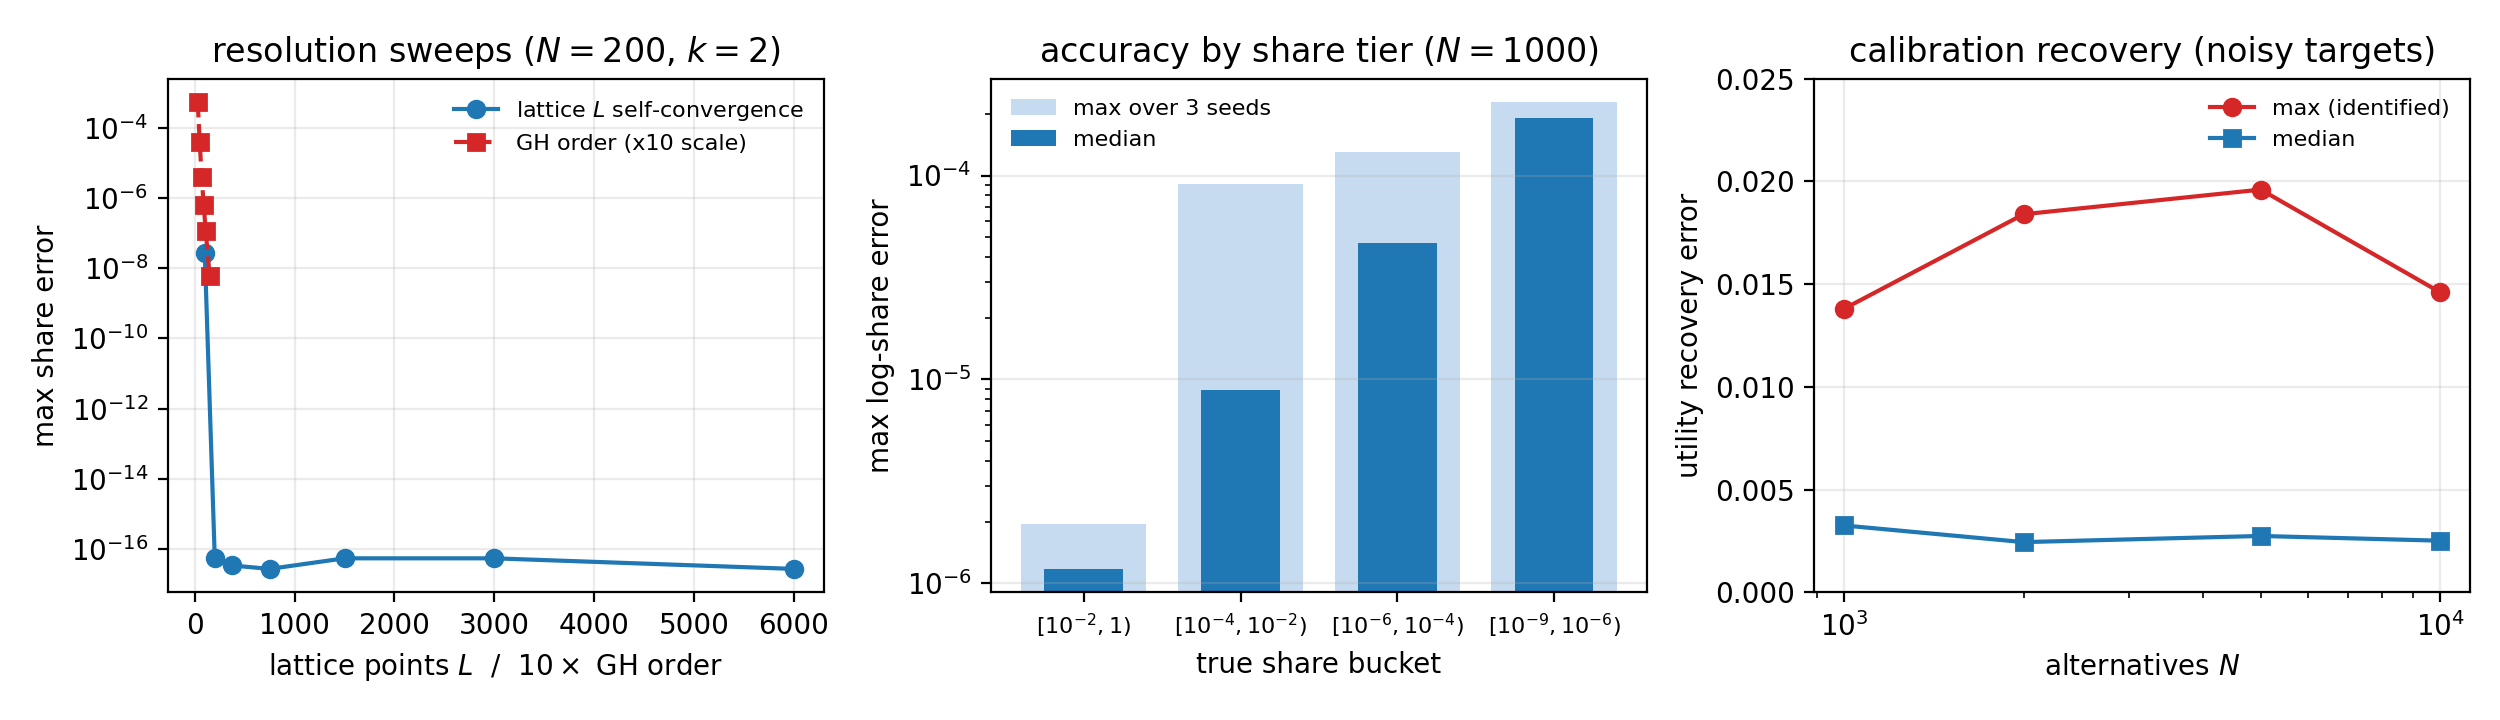
\includegraphics[width=\textwidth]{figs/validation.png}
\caption{Central validation evidence, from the experiments.
Left: lattice self-convergence in $L$ and Gauss--Hermite factor sweep
(experiment 17). Middle: log-share error against higher-resolution internal
references by true-share bucket at $N = 1000$, three problems
(experiment 25). Right: utility recovery against independent
$5\times10^6$-draw noisy targets over $N = 1000$ to $10000$
(experiment 19); the plateau is target sampling noise, not solver error
(experiment 21).}
\label{fig:validation}
\end{figure}

\paragraph{Resolution sweeps.} Figure~\ref{fig:validation} collects the
central accuracy evidence. Experiment 17 sweeps
each resolution knob separately at $N=200$, $k=2$.
Holding the factor rule fixed, lattice self-convergence is
$2.7\times10^{-8}$ at $L=101$ and at machine precision from $L \approx
200$. The convergence observed over the tested range is
near-exponential. For these analytic, rapidly decaying integrands the
lattice error becomes negligible very quickly, leaving the $L$-error
subdominant.

Holding $L$
fixed, the Gauss--Hermite sweep decays from $5.3\times10^{-4}$ (order 3) to
$5.9\times10^{-9}$ (order 15).

\paragraph{Experimental errors.} Empirical convergence evidence is not a rigorous proof, and we still rely on it in part. The error sources separate cleanly by status:

\begin{center}
\footnotesize
\begin{tabular}{lp{6.2cm}}
\toprule
error source & status \\
\midrule
factor-node pruning & rigorous bound ($\delta$ sup-norm) \\
finite envelope & rigorous bound ($N\Phi(-8)$) \\
covariance approximation & rigorous Kullback--Leibler (KL)/Pinsker bound (Section~\ref{sec:boundary}) \\
$x$-grid discretization & empirical convergence assessment \\
factor quadrature & empirical higher-order comparison \\
calibration residual & directly measured solver consistency \\
\bottomrule
\end{tabular}
\end{center}

\paragraph{Stability checks and two genuine bounds.} Self-convergence
checks at large $N$ show stability below what the
simulation references can resolve: refining to $(L = 3001, \mathrm{GH}21)$
moves the shares by $1.2\times10^{-8}$ at $N=1000$ and
$5.7\times10^{-8}$ at $N=5000$. This is a stability statement, not by
itself an error bound, since both resolutions could share bias.

Two genuine bounds
come free from the product structure. Conditional probabilities lie in
$[0,1]$, so pruning factor weight $\delta$ perturbs unnormalized shares by
at most $\delta = 2.39\times10^{-8}$ in sup norm (measured
$6.2\times10^{-9}$). The $\pm8\sigma_{\max}$ envelope omits
conditional mass at most $N\Phi(-8) + \Phi(-8)^N \le (N+1)\Phi(-8)
\approx 6\times10^{-12}$ even at $N = 10^4$ (conditional on each retained factor node, the lower tail by a union
bound and the upper by conditional independence).

\paragraph{Calibration accuracy at $N=1000$.}

At $N=1000$, $k=2$, with targets from
$5\times10^6$ MC draws floored at $10^{-7}$ and renormalized, the inversion
completes in about three seconds in the compiled implementation. The
iteration solves its own equations
to $6.4\times10^{-9}$. This is a statement about the solver, not
statistical accuracy, since the target carries sampling noise near
$2\times10^{-4}$. It recovers the utilities
of the well-resolved alternatives (target share above $3\times10^{-4}$)
to maximum error $0.017$.

A replication study (experiment
16) repeats the inversion on a second $N=1000$ problem against three
independent $5\times10^6$-draw targets: 161--162
alternatives well-resolved (98.1\% of share mass), recovery error maximum
$0.015$--$0.023$ and median $\approx 0.0027$ across replicates, with the
recovery-versus-share curve reported alongside.

\paragraph{Validation: where the error comes from.} Experiment 21
separates the error sources. A noiseless inverse
test (targets generated by the lattice map itself, a deliberate inverse
crime that isolates solver plumbing) recovers the utilities of every
resolvable alternative to $6.5\times10^{-7}$ at $N=200$ and
$1.2\times10^{-7}$ at $N=1000$---solver error at the tolerance, so the
$\approx 0.02$ recovery in noisy tests is the targets' sampling noise
showing through. Alternatives with shares below the resolution floor are not
chased, by design. Their tier is reported separately.

\paragraph{Independent inversion validation.} Experiment 35 closes the
gap between noisy simulation references and same-method lattice
references. Target shares at $N = 50$, $100$, and $200$ are generated
by the per-alternative factor-conditioned RQMC integral of
Section~\ref{sec:comparisons} at $2^{17}$ scrambled-Sobol points,
sharing no code path with the lattice, and the lattice calibration then
inverts them. Utilities are identified up to location, and the tail
coordinates carry the targets' absolute-error floor of about $10^{-5}$,
so recovery is scored after recentering on the well-resolved set. On
shares above $10^{-2}$ the recovered utilities match the truth to
$7.6\times10^{-5}$, $1.1\times10^{-4}$, and $3.0\times10^{-4}$ at the
three sizes, with medians $1.3\times10^{-5}$ to $6.8\times10^{-5}$. On
shares above $10^{-3}$ the maximum is about $10^{-3}$, which is the
targets' own relative accuracy at that share level. The recovery floor
tracks the reference, not the solver.

\paragraph{Robustness.} Twenty problems that vary utility spread, factor
strength, $D$-heterogeneity, and rank all converged (6--31 iterations, recovery
$0.004$--$0.024$).

A further stress test targets heterogeneous idiosyncratic variances,
where the common envelope is set by the largest $\sqrt{D_i}$ while the
narrowest conditional density can approach the grid spacing. At
variance ratio $10^2$ the production lattice is already converged
(log-share agreement $5\times10^{-12}$ against $L = 8001$). At ratio
$10^3$ the production $L = 501$ carries a maximum log-share error of
$1.0\times10^{-3}$, and $L = 2001$ restores machine precision
(experiment 33). The practical rule is to scale $L$ with the ratio of
envelope width to the smallest conditional scale.

The assembled numerical Jacobian has the symmetry, row-sum, and
reduced positive-definiteness properties predicted by
Proposition~\ref{thm:inv}. The reduced Jacobian assembled from $N$
Jacobian--vector-product calls
at $N=50$ is symmetric to $1.7\times10^{-18}$ (an assembly identity,
tighter than the finite-difference symmetry check of
Section~\ref{sec:structure}), has row-sum defect
$6.2\times10^{-17}$, and reduced eigenvalues in $[2.5\times10^{-5},
0.22]$, positive definite as proved.

\paragraph{Compiled implementation.} The same pass in Rust (in the
repository, with machine-precision parity and identical iteration counts)
calibrates $N=1000$ in 3 seconds, $N=5000$ in 18 seconds, and
$N=10000$ in 38 seconds (10, 11, and 13 iterations; independent
$5\times10^6$-draw targets, experiment 19).

\paragraph{Scaling.} Calibration is approximately linear in $N$ over
the tested range (experiment 19), flat at 11--15
forward-pass equivalents of total wall time throughout (the excess over
the iteration count is the warm start), with recovery quality unchanged
(median error near $0.003$, 96--99\% of share mass identified). At fixed
spatial resolution the cost grows slowly with the utility range,
$O(\sqrt{\log N})$ under Gaussian utilities.

Figure~\ref{fig:scaling} shows calibration wall time growing roughly
linearly in the number of alternatives.

\begin{figure}[t]
\centering
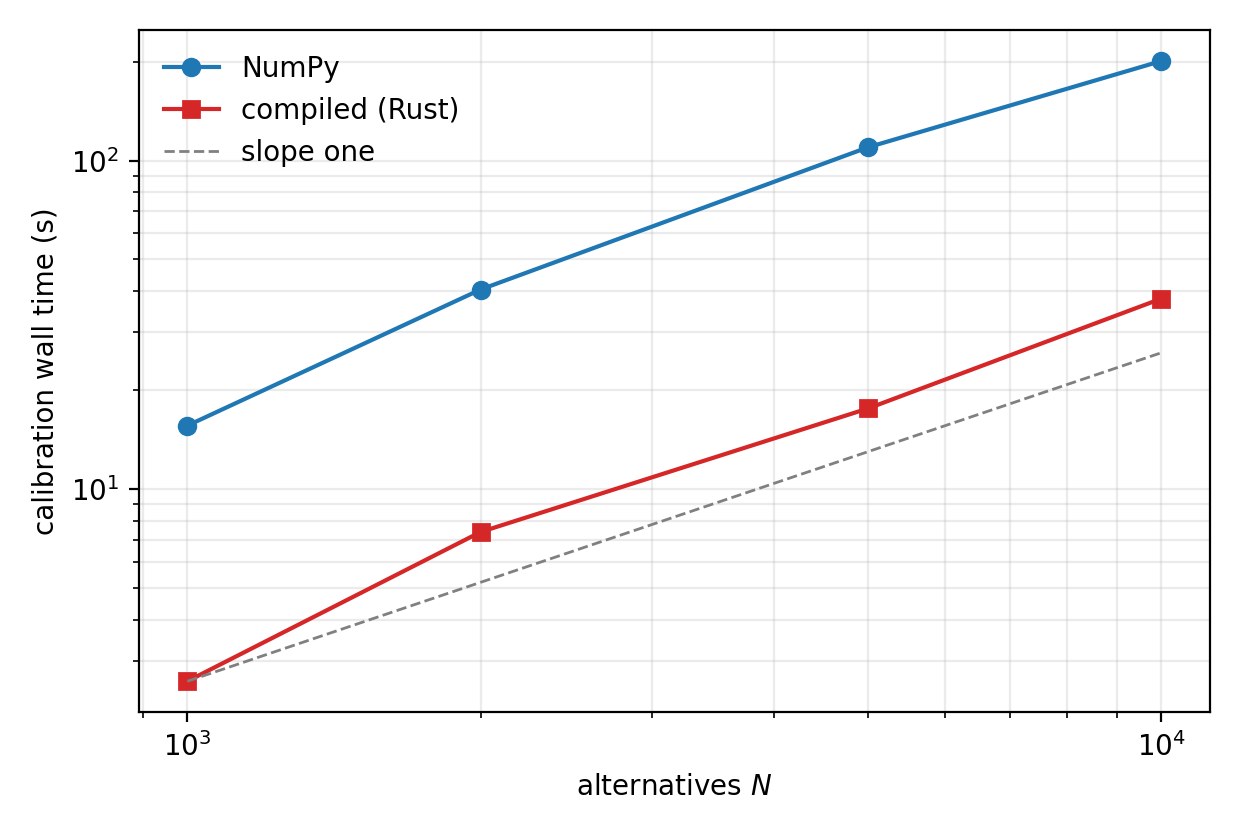
\includegraphics[width=0.62\textwidth]{figs/calibration_scaling.png}
\caption{Wall time to calibrate the full utility vector from target
shares ($k=2$ factors, independent $5\times10^6$-draw targets, experiment
19). Both implementations grow roughly linearly in $N$. The dashed guide
has slope one. Recovery accuracy is assessed on alternatives above the
share-resolution threshold.}
\label{fig:scaling}
\end{figure}

\paragraph{Derivatives.} For fixed factor nodes and a fixed
lattice, the transform is a reproducible, (piecewise-)differentiable function
of $\mu$ whose derivatives are evaluated without resampling. The analytic own-location slopes of the unnormalized map come from the same pass and serve as the inversion preconditioner. Along a utility path at $N=50$, the maximum second difference over
$dt^2$ is 39.3 for fresh-draw GHK against 0.01 for both GHK under common
random numbers (CRN-GHK) and the lattice. The curves are in the
committed output.

These are derivatives of the numerical
approximation, not exact MNP derivatives, and GHK-based practice likewise
differentiates its approximation, analytically or with fixed draws
\citep{hmr1996,hajivassiliou1998,train2009}. The practical distinction is the character and controllability of the
approximation error, quadrature resolution versus draw count, not the
possibility of differentiation.

\paragraph{Estimation gradients (by-product).} Experiment 30
parameterizes the covariance, $V(\theta) = \theta_1 V_0$ and
$D(\theta) = e^{\theta_2} D_0$, across four markets that share one
utility vector and differ by known factor-scale multipliers. The outer
objective is the cross-market disagreement of the calibrated utilities,
$\mathcal{L}(\theta) = \sum_m \|\mu_m(\theta) - \bar\mu(\theta)\|^2$, which
vanishes at the truth. This is a cross-market restriction of the kind
that disciplines the covariance where a single menu cannot. The
gradient passes through the calibration fixed point by the implicit
function theorem, $d\mu/d\theta = -B(B^\top J B)^{-1}B^\top\,
\partial p/\partial\theta$. In this experiment the reduced Jacobian is
assembled by symmetrized central differences and solved densely at
$N = 50$. The matrix-free route through Proposition~\ref{prop:jvp} is
the large-$N$ substitute. The implicit gradient matches central finite
differences of the objective to $1.2\times10^{-7}$, and a damped Newton
outer loop converges in three iterations to the truth up to the probit
scale gauge (recovered $\theta_1^2 e^{-\theta_2} = 1.0000000$ against
$1$), which shares cannot identify. The scale ambiguity emerges from
the experiment rather than being imposed.

\paragraph{Removal ensemble (by-product).} The cached field also yields
all $N$ single-removal share vectors in $O(QN^2L)$, at roughly a third
the wall time of recomputing them from scratch at $N=200$.

Against the strongest simulation comparator, which reuses each draw's
winner and runner-up to answer every removal at once in $O(RN + N^2)$, the
deterministic ensemble is about $4.5\times$ more accurate at matched wall
time at $N=200$ ($4.2\times10^{-5}$ versus $1.9\times10^{-4}$;
experiment 18).\footnote{This is a side capability, not the paper's calibration emphasis.}

\section{Further structure}\label{sec:structure}

This section records interpretations that connect the map of
Section~\ref{sec:theory} to older mathematics. Nothing downstream
depends on them.

\paragraph{Relation to the multiplicity calculus.} The photo-finish weight
is the differentiated form of the \emph{multiplicity} that the original
transform \citep{cotton2021} tracks in the forward direction. There the
multiplicity is a scalar field on the lattice: the expected number of
runners sharing the winning cell, needed to split dead-heat payoffs,
since an $m$-way tie pays each winner $1/m$.

Multiplicity so defined is the expectation of a discrete count. Its
excess over one is $O(\Delta x)$ in the cell width and vanishes as
the lattice refines. The weight $w_{ij}$ is the continuum, pairwise
density of the same event, a two-way tie between $i$ and $j$ with the
rest behind, and it survives the continuum limit because
$-w_{ij} = \partial p_i/\partial\mu_j$ is a rate rather than a count. The
two are one identity apart: the multiplicity's excess over one, per unit
lattice spacing, is the total tie density
\[
\sum_{i<j} w_{ij} \;=\; \tfrac12\,\mathrm{tr}(J),
\]
which experiment~37 confirms---the measured excess-over-one divided by
the cell width converges to $\tfrac12\,\mathrm{tr}(J)$ as
$\Delta x \to 0$. The forward pass counts ties to divide payoffs.
Calibration differentiates them into the graph-Laplacian weights that
make it a network solve.

\paragraph{The conjugate view.} Here we lean on social-surplus convex
duality for discrete choice \citep{chiong2016,norets2013}. Our
contribution is the algorithm, not the well-posedness of the inversion,
which is known. $G$ is
convex with $p = \nabla G$, so $\Omega = G^*$ is a convex regularizer on
the simplex and $p(\mu) = \arg\max_{q \in \Delta}\{\mu^\top q -
\Omega(q)\}$. For i.i.d.\ Gumbel noise $\Omega$ is Shannon negentropy and
the maximizer is softmax. In general it is the generalized entropy of
\citet{fosgerau2020}, with the perturbation--regularization duality
developed for machine learning by \citet{berthet2020}.
\citet{melo2025} gives the online-learning reading of the same
duality. Factor probit
carries a covariance-dependent, non-separable entropy that couples
alternatives through the factor structure. 

In this paper we give three
algorithms, and they could be thought of as three faces of that dual
pair. The transform evaluates $\nabla G$. Calibration evaluates the
mirror map $\mu = \nabla\Omega(p)$ on the mean-zero quotient. The
Jacobian--vector product applies the Hessian $\nabla^2 G$. Each is
built from the same $O(QN(k+L))$ primitive. The forward map is one
pass, each Jacobian--vector product is one pass, and each calibration
iteration is one pass (total calibration cost multiplies by the
iteration count, typically 10--15). 

On the simplex, $\nabla\Omega(p)$ is an equivalence
class modulo constants. Its mean-zero representative is the calibrated
utility. The bijection itself is essentially known
\citep{hotz1993,norets2013,bgh2013}, with the attributions detailed in
Section~\ref{sec:related}. The connectivity mechanism of
\citet{bgh2013} is the photo-finish graph's. The appendix proof (Appendix~\ref{app:inv}) keeps the
Gaussian factor case self-contained and exhibits the weights the algorithm uses. Each
identity in the proposition is also checked
numerically in the repository: the $w_{ij}$ representation against finite
differences to $6\times10^{-9}$, symmetry to $4\times10^{-12}$, and
positive definiteness of the reduced numerical Jacobian.


\paragraph{Transport form.}

There is another interpretation. On the contrast space, with $b_i = e_i - \mathbf{1}/N$ the vertices of
a regular simplex, $\arg\max_i (x_i + \mu_i) = \arg\min_i
\{\tfrac12 \|x - b_i\|^2 - \mu_i\}$: the choice cells are the
Laguerre cells of quadratic semi-discrete optimal transport from the
contrast Gaussian (the law of $P\xi$, $P = I - \mathbf{1}\mathbf{1}^\top/N$) to $\nu_q = \sum_i q_i \delta_{b_i}$, and
Kantorovich duality identifies $\Omega(q)$, up to an additive constant,
with $\tfrac12 W_2^2$ between them. Calibration is the dual solve of a
structured transport problem. The weight $w_{ij}$ is the Gaussian surface
mass on the shared Laguerre facet (scaled by $1/\sqrt2$), and a Newton step is
an electrical solve on that network, for which
Proposition~\ref{prop:jvp} is the matrix-free multiply.%
\footnote{Place the alternatives as the corners of a
regular simplex, and let each Gaussian draw pick its nearest corner,
where corner $i$'s reach is enlarged or shrunk by its utility $\mu_i$.
The choice regions are then the cells of a power diagram (a weighted
Voronoi tessellation), and a choice probability is the Gaussian mass
that falls in a cell. Calibration---nudging the utilities until each
cell captures its target share $q_i$---is the semi-discrete
optimal-transport problem of moving the Gaussian mass onto the corners
at minimum squared-distance cost, with the utilities acting as transport
prices and $\Omega$ as the transport cost. The weight $w_{ij}$ is the
Gaussian mass on the wall between cells $i$ and $j$; a Newton step pours
the share residuals into the nodes as currents, treats those
wall-masses as conductances, and solves for utility corrections as
voltages, which Proposition~\ref{prop:jvp} performs without forming the
matrix.}

The geometry above is standard semi-discrete optimal transport. The
power-diagram formulation goes back to \citet{aurenhammer1998}.
\citet{levy2015} optimizes the weights through a convex objective.
\citet{kmt2019} analyze a damped Newton method whose Hessian is a
weighted graph Laplacian with facet-integral weights, with global
convergence under regularity and support conditions that an unbounded
Gaussian source does not immediately satisfy. \citet{taskesen2023}
connect discrete-choice smoothing and semi-discrete transport directly.
What is new here is the evaluation primitive. The factor structure gives an
$O(QN(k+L))$ evaluation of all cell masses at once, and of
Hessian--vector products without facet enumeration, when the source is
a factor Gaussian and the sites are the simplex vertices.

At calibrated utilities the conjugate value admits a trace evaluation
identity. The identity is a factor-probit specialization of Gaussian
integration by parts, Stein's identity \citep{stein1981}. Its useful
content here is the photo-finish decomposition and the fact that the
same matrix-free primitives the calibration uses evaluate it.

\begin{proposition}[Conjugate trace identity]\label{prop:trace}
For model \eqref{eq:model}, with $J = J(\mu)$ and $p = p(\mu)$,
\[
G(\mu) = \mu^\top p + \mathrm{tr}(\Sigma J),
\qquad
\Omega(p) = -\mathrm{tr}(\Sigma J)
= -\sum_{i<j} w_{ij}\, s_{ij}^2, \qquad
s_{ij}^2 = D_i + D_j + \|v_i - v_j\|^2 .
\]
\end{proposition}
\begin{proof}[Sketch]
$G - \mu^\top p = \E[\xi_I]$, the mean shock of the winner. The
divergence theorem turns each choice cell's contribution into Gaussian
facet integrals, and the facet masses are the photo-finish weights
$w_{ij}$. Summing gives $\mathrm{tr}(\Sigma J)$.
Appendix~\ref{app:trace} carries out the steps.
\end{proof}
Read the graph
as a network of wires: $w_{ij}$ is the conductance of
edge $ij$, and $s_{ij}^2 = \operatorname{Var}(U_i - U_j)$ is the noise in the
$i$-versus-$j$ race. The entropy $\Omega$ is minus the total
conductance, each edge weighted by its noise. Only differences $v_i -
v_j$ and sums $D_i + D_j$ appear, so adding a common part to the
covariance leaves $\Omega$ unchanged. Only the contrast part
$P\Sigma P$ of the covariance can matter, a property
Section~\ref{sec:comparisons} develops for covariance fitting.

We checked this in the code (see experiment 27 in particular). The
binary closed form $\Omega = -s\,\phi(\Phi^{-1}(q))$, with $s^2$ the
difference variance and $q$ the first share, is verified to
$3\times10^{-13}$. The full identity is verified to $3\times10^{-9}$. That $G^*$ is an assignment problem was already known \citep{chiong2016}; new here is the simplex form and also the
evaluation of the conjugate value
at calibrated utilities from $k$ Jacobian--vector products and the
diagonal slopes. The gradient $\nabla\Omega(p) = \mu$ is dearer. It
requires the calibration solve, and Hessian actions of $\Omega$ require
reduced linear solves built from the same Jacobian--vector products.


\section{Related work}\label{sec:related}

\paragraph{Prior art.} The nearest methods, and what each lacks:
\nopagebreak[4]

\begin{center}
\footnotesize
\setlength{\tabcolsep}{5pt}
\renewcommand{\arraystretch}{1.25}
\begin{tabular}{|p{4.1cm}|p{4.1cm}|p{4.5cm}|}
\hline
\textbf{approach} & \textbf{all $N$ shares} & \textbf{calibration} \\
\hline
GHK simulation \citep{geweke1994,hajivassiliou1998} & $N$ separate runs, $R^{-1/2}$ (plain MC) & no reported large-$N$ share inversion known to us \\
\hline
direct utility simulation & whole vector per draw, $R^{-1/2}$ & raw frequency map is nonsmooth \\
\hline
analytic approximations \citep{bhat2011,connors2014} & per-alternative & not provided \\
\hline
factor quadrature \citep{butler1982,elrod1995} & $N$ separate $(k{+}1)$-dim integrals & not provided \\
\hline
Bayesian factor MNP \citep{loaiza2022} & simulation inside estimation & posterior, not a share map \\
\hline
neural amortization \citep{huch2026} & learned approximation, accuracy not resolution-controlled & not provided \\
\hline
BLP-side inversion \citep{berry1995,conlon2020} & --- & logit family only \\
\hline
\textbf{this paper} & one $O(QNL)$ pass & Prop.~\ref{thm:inv}; 3\,s at $N{=}1000$ (compiled) \\
\hline
\end{tabular}
\end{center}



GHK and simulated likelihood are standard in econometrics
\citep{geweke1994,hajivassiliou1998,train2009}, with
\citet{hmr1996} the standard treatment of simulated multivariate
normal (MVN) probabilities
and their derivatives; \citet{genz1992}
developed the same separation-of-variables construction in numerical
statistics, where its RQMC form is the default MVN evaluator, anchored
by the Genz--Bretz book \citep{genzbretz2009} and the \texttt{mvtnorm}
package \citep{mi2009}.

Deterministic grid recursions exist within that ecosystem: \citet{miwa2003}
evaluate orthant probabilities by recursion on one-dimensional lattices,
at factorial cost in the dimension for general correlation, and
\citet{craig2008} accelerates the Markov case; both price one
probability per run. \citet{ridgway2016} reads GHK as sequential importance sampling, proves its
variance can deteriorate exponentially, and builds sequential Monte
Carlo (SMC) alternatives. \citet{botev2017} sharpened the family with
minimax tilting, and \citet{genton2018} began the hierarchical line in
this journal. \citet{cao2021} push MVN probabilities to thousands of
dimensions with tile-low-rank QMC, machinery pointed almost exactly at
our difference covariances, which are diagonal plus rank $k+1$.
\citet{cao2025} reach linear per-probability cost past twenty thousand
dimensions with Vecchia approximations.

Deterministic approximations run from Mendell--Elston \citep{mendell1974}
(surprisingly competitive when optimally ordered \citep{connors2014})
through Bhat's MACML \citep{bhat2011} to expectation propagation:
\citet{cunningham2011} found EP
highly accurate precisely for rectangular regions, and \citet{fasano2025} evaluate generic Gaussian CDFs by EP on a dual probit
model, deterministically and sampling-free. Every one of these prices one
orthant at a time. None couples the $N$ winner probabilities.

Factor dimension reduction for probit is old, and older than
econometrics: \citet{curnow1962} showed that product correlation
collapses the multivariate normal integral to a one-dimensional integral
of products of univariate CDFs, the reduction this paper conditions on,
and \citet{dunnett1989} is its standard algorithm. The ranking-and-selection
tradition built on the same integrals from the 1950s
\citep{bechhofer1954,gupta1963}, always evaluating one designated
candidate per integral: assembling all $N$ that way costs $N$ separate
integrals where the shared field gives all $N$ in one pass.

In
econometrics, \citet{butler1982} integrated one factor by quadrature,
and \citet{lee2000} stabilized that quadrature numerically;
\citet{mcfadden1984} proposed factor-analytic MNP expressly as dimension
reduction; \citet{stern1992} used the same conditional-independence
product of normal CDFs with Monte Carlo over the residual;
\citet{bolduc1999} handled large choice sets with parsimonious
covariances but simulated probabilities. Sparse-grid integration
\citep{heiss2008} attacks the rank growth that binds product rules.

\citet{elrod1995}
estimated factor-analytic probit for panel data;
\citet{haaijer1998} estimated utility covariances in conjoint MNP;
\citet{cohen2010} built a structured covariance probit expressly for
demand estimation;
\citet{loaiza2022} pursue large choice sets by
Bayesian estimation, with variational follow-ups \citep{loaiza2023};
\citet{kim2026} reach twenty alternatives at a million observations by
neural variational inference, and \citet{ding2024} exceed a hundred with
expectation-propagation E-steps. All are approximate forward maps for
estimation, and none inverts shares. \citet{girolami2006} use the
one-dimensional product identity in its diagonal-covariance form,
per class. \citet{collier2021} place the factor-Gaussian race with
low-rank-plus-diagonal covariance on the last layer of large-scale image
classifiers, including thousand-class ImageNet, and approximate the
winner probabilities by Monte Carlo over a temperature-softmax
relaxation; \citet{berthet2020} differentiate general perturbed-argmax
layers by Monte Carlo, with $p = \nabla G$ as the organizing identity.
Both simulate the map this paper evaluates deterministically.

Racing supplied two of our ingredients. \citet{henery1981} wrote the
survival-product win integral for normal running times and gave its
first-order analytic inversion. \citet{ali1998} inverted market odds to
abilities numerically at eight-runner fields, and betting practice
otherwise approximated the inversion away \citep{lo1994}. The lattice survival-product identity and
its fast inverse transform come from racing \citep{cotton2021} and ship in
the \texttt{winning} package \citep{winningpkg}. \citet{cotton2021}
names the common-factor extension developed here as an open problem.

The shared-product assembly itself also appears in competing-risks
computation: \citet{mahani2019} compute all cause-specific cumulative
incidences on one shared grid by forming the product of every survival
function once and dividing out each cause's own factor (software since
2015), and the Aalen--Johansen estimator \citep{aalen1978} reads all
causes off a single survival product nonparametrically. Neither embeds
the assembly in factor quadrature, differentiates it, nor inverts it.
Racing arrived at it independently.

An older transportation literature used ``calibration'' for MNP
parameter estimation. \citet{daganzo1977} introduced an early numerical
MNP forecasting algorithm and claimed applicability to large problems,
with \citet{daganzo1979} the monograph treatment;
\citet{sheffi1982} reviewed probability and calibration methods and
proposed simulation-based estimation; \citet{kamakura1989} embedded the
Mendell--Elston approximation in a calibration routine. These estimate
parameters from choice data or approximate designated probabilities;
none provides a smooth all-$N$ share map, a shared-field
Jacobian--vector product, or aggregate-share inversion at the scale
considered here.

Inversion theory is likewise established. \citet{berry1994} made
share-to-utility inversion the workhorse of demand estimation;
\citet{bonnet2022} invert demand in general, including nonsmooth
random-utility models, through two-sided matching;
\citet{hotz1993}
inverted choice probabilities to utility differences; \citet{norets2013}
prove surjectivity of the utility-to-probability map;
\citet{bgh2013} obtain demand invertibility from
connected substitution;
\citet{chiong2016} invert through the convex
conjugate; \citet{fosgerau2020} show the probit inverse exists by
generalized-entropy duality, without an algorithm.

 \citet{berry1995} built demand
estimation on the logit-side inversion, and \citet{conlon2020}
maintain its modern practice. \citet{chia2021}
differentiates logit BLP automatically. On the generalized extreme value (GEV) side, closed-form
flexible-correlation kernels pursue rich substitution without
high-dimensional integration \citep{tinessa2020,tinessa2021}.
Meanwhile \citet{huch2026}
amortize correlated-choice probabilities with neural networks, evidence of
current demand for this computation.

The novelty here is accordingly not dimension reduction
\citep{curnow1962}, nor the order-statistic integral, nor the
shared-product assembly in isolation \citep{mahani2019,cotton2021}, nor
well-posedness of inversion. It is the
all-alternatives assembly in $O(QNL)$, its large-$N$ implementation, the
$O(QNL)$ Jacobian--vector product, and the shared-field reuse for
calibration and counterfactuals. Convenient error partitioning
\citep{train1995} integrates part of the noise away for one designated
alternative at a time. The shared field recognizes that the $N$
resulting integrands share one product and computes the whole vector
together.

\section{Comparisons with existing algorithms}\label{sec:comparisons}
\label{sec:boundary}

We now compare with existing approaches: first the natural
factor-aware competitor, then simulation in its weakest and strongest
forms, then the boundary regimes where the factor form itself, rather
than the numerics, is the binding approximation, and finally the
substitution experiments that measure what logit's restriction costs.

\paragraph{The natural competitor.} Conditioning on the factors and the alternative's own shock makes each
probability a $(k{+}1)$-dimensional integral,
\[
p_i = \E_{f,z} \prod_{j \ne i}
\Phi\!\left(\frac{\mu_i - \mu_j + (v_i - v_j)^\top f +
\sqrt{D_i}\,z}{\sqrt{D_j}}\right),
\]
evaluable per alternative by modern randomized quasi-Monte Carlo: the
natural competitor that uses exactly the structure this paper assumes.
The conditioning idea is the \emph{convenient error partitioning} of \citet{train1995}, which conditions on components common across
alternatives and computes what remains analytically. It
still prices $N$ separate integrals, $O(RN^2)$ in total, where the shared
field couples them into one $O(QN(k+L))$ pass. Measured at matched
$4\times10^{-4}$ accuracy (experiment 24; the two implementations first
verified against each other to $1.7\times10^{-5}$), the per-alternative
route is about $140\times$ slower than the single shared-field pass at
$N = 1000$, a gap that widens linearly in $N$.
Both implementations are NumPy on the same machine.

\paragraph{The price of smoothness.} Smoothness was never a side
issue in this literature. It shaped it. The raw frequency simulator is a
step function of the parameters, so \citet{stern1992} accepted a large
per-draw cost purely to smooth it, and GHK's adoption owed as much to
producing smooth, positive, differentiable estimates
\citep{hajivassiliou1998} as to its variance reduction. The lattice ends
that trade. It is smooth to resolution, and its derivatives are exact
integrals of the same pass, so the property the simulation literature
paid variance and wall time for costs nothing here.

\paragraph{The limits of winner-frequency simulation.} With common
random numbers a smoothed simulator such as CRN-GHK is a fixed function
that a solver can match to fine tolerance (a raw draw-and-argmax map is
piecewise constant on the $1/R$ grid and cannot be). The limitation is
not smoothness. It is the error of that fixed function against the
exact map, and the cost of driving it down.

Its coordinatewise error against the exact map is of order
$\sqrt{p_{\max}/R}$, so making the simulated map itself $\tau$-accurate
costs $R \approx p_{\max}/\tau^2$ independent draws per evaluation, and
inverting it exactly still leaves utilities whose true shares miss the
target at a scale that is order $\tau$ but amplified through $J^{-1}$.

If we take the example of crude winner-frequency simulation with $N = 5000$, this
means driving the simulator to the solver's consistency level, $\tau
\sim 10^{-6}$, well beyond the $2\times10^{-4}$ statistical accuracy of the
noisy-target experiments. At that scale each forward evaluation needs
$R \approx p_{\max}/\tau^2$ draws, which at the direct-simulation
throughputs we measured is weeks of computation. A calibration could
take months to a year. 

If calibration time at a fixed accuracy can be reduced from months to
a few seconds, the tradeoff between probit and its analytically simpler logit
cousin changes. This particular example is roughly a six-order-of-magnitude speedup. 

Common random numbers do not change the plain-MC rate. Randomized QMC and
specialized Gaussian integration can improve rates as well as
constants. The structural gap is different: per-alternative
formulations price $N$ separate integrals whose integrands each carry
$O(N)$ factors, and the shared field removes that factor of $N$. A
maximum over $N$ coordinates adds a further $\log N$ factor in
high-probability statements.

Returning to winner-frequency calibration, at the crude
$\tau = 10^{-4}$ where simulation-in-the-loop first becomes feasible, the calibrated model's true
shares miss the target at $10^{-4}$ and the answer moves with each set of samples. 

In contrast the quadrature route's accuracy against the exact map is set by
resolution, not draws, at cost independent of $\tau$ until resolution
binds. We are unaware of a reported
probit share inversion at this scale in simulation-based practice, and this
scaling is presumably why. Within the fixed low-factor regime, that constraint is now gone. 



\paragraph{The strongest simple simulator.} Simulation can do much
better than winner frequencies at no structural cost, again following
\citet{train1995}. Draw the factors
and every idiosyncratic shock, form each alternative's best rival
$M_{-i} = \max_{j \ne i} U_j$ (all $N$ of them from the top-two
statistics, in $O(N)$ per draw), and average $\Phi((\mu_i + v_i^\top
f - M_{-i})/\sqrt{D_i})$. The estimator is unbiased coordinatewise,
smooth apart from max-switch kinks, and $O(RN)$ for the whole vector.
Measured at $N = 200$ (experiment 38), at $R = 10^5$ it beats winner
frequencies by roughly $3\times$ in maximum absolute error and
$6\times$ in total variation ($3.2\times10^{-4}$ and
$1.4\times10^{-3}$). Its best log-share error on shares above $10^{-3}$
is $1.8\times10^{-2}$, against about $10^{-4}$ for the lattice at
comparable sizes. Conditioning improves the absolute scale but not the relative accuracy
of small shares, and calibration needs the latter.

A smooth all-$N$ comparator from machine learning is the
temperature-softmax relaxation $\E[\mathrm{softmax}((\mu + \xi)/T)]$
with common draws \citep{collier2021,berthet2020}, computing every
share in $O(RN)$. It is biased at any fixed temperature and noisy at
finite draws. Measured at $N = 200$ against the lattice map (experiment
34), its best settings over $T \in [0.03, 1]$ and $R \le 2\times10^5$
leave a maximum absolute share error above $9\times10^{-4}$ and
log-share errors above $0.1$ on shares over $10^{-3}$, with total
variation $0.43$ at $T = 1$. Sharpening $T$ trades bias for variance.
The lattice's corresponding log-share error is below about $10^{-4}$
at the sizes bracketing $N = 200$ measured in experiment 25.

\paragraph{General covariance through the factor approximation.} 

To use the method when $\Sigma$ is general, one first fits a factor
model. Absolute utility levels are arbitrary, just as only relative
horse ability matters in a race, and failing to account for this can
``waste'' factors. 

To be more formal, the method
requires $\Sigma \approx VV^\top + \mathrm{diag}(D)$. GHK does not. Choices depend on
$(\mu, \Sigma)$ only through $P\mu$ and $P\Sigma P$, $P = I -
\mathbf{1}\mathbf{1}^\top/N$, because the argmax is determined by
pairwise differences. So a common factor loading $V \to V +
\mathbf{1}c^\top$ shifts every conditional location equally and cannot move
the argmax (a machine-precision identity). 

Our advice is that a factor fit must be run in a choice-relevant
quotient space. In contrast, fitting raw $\Sigma$ can spend
scarce rank on an irrelevant common component ($\Sigma = \kappa^2
\mathbf{1}\mathbf{1}^\top + \beta\beta^\top + \mathrm{diag}(D)$ with large $\kappa$: the
raw rank-1 fit takes $\mathbf{1}\mathbf{1}^\top$ and misses
$\beta\beta^\top$ entirely; on such an example the contrast-space fit cuts
rank-1 share error from $4.6\times10^{-2}$ to $8.3\times10^{-3}$).

The asymmetry matters. Only the common \emph{factor} direction is
irrelevant. A common addition to $D$ inflates every difference variance
and is choice-relevant, so $D$ must come from the quotient fit.

The suggested fit is an iterative principal-factor heuristic applied to $P\Sigma P$ (eigendecompose
$P\Sigma P - \mathrm{diag}(D)$, take the top $k$ directions, refit $D$ from
the diagonal with a $10^{-3}$ floor, iterate to $10^{-10}$), followed by
centering and singular value decomposition (SVD) canonicalization of the loadings (ordered columns, fixed
signs).

This procedure will not, however, minimize a projected norm
($P\,\mathrm{diag}(D)\,P$ is not diagonal). Therefore the repository also implements an alternating least-squares fit with
exact block updates on the reduced quotient (precisely, a top-$k$ positive semidefinite (PSD) step for the
loadings and a nonnegative least squares for $D$ that is exact block
minimization but should not be interpreted as global optimality). On
the boundary matrices it changes the quotient residual by under 1\%.

The covariance-quotient residual $\|P(\Sigma -
\hat\Sigma)P\|_F / \|P\Sigma P\|_F$ is reported alongside every share
error in the committed output.

We test this approach on correlation matrices with spectral decay
$\lambda_m \propto m^{-\gamma}$, $\gamma \in \{0.5, 1.5, 3\}$, at
$N=50$ (sharing one
orthogonal eigenbasis across $\gamma$ so decay comparisons are not
confounded with basis realization). The power law holds before diagonal
standardization, which perturbs the spectrum; the actual leading eigenvalues
(3.7, 17.1, 34.2 at $\gamma = 0.5, 1.5, 3$) are printed by the script.

Share error is measured against an $8\times10^6$-draw reference, with GHK
at the exact $\Sigma$ for comparison. The plotted quantity is the rank-$k$
approximation error of the stated procedure, not a minimum over factor
models.

Rank-8 errors: $1.8\times10^{-3}$, $3.7\times10^{-3}$, and
$3.1\times10^{-3}$ at $\gamma = 0.5, 1.5, 3$ from $k=1$ starting points of
$2.3\times10^{-3}$, $1.5\times10^{-2}$, $7.1\times10^{-2}$.

The lattice versus simulation discrepancy is also tested. We simulate
under the \emph{fitted} factor model $\hat\Sigma$ and compare with the
lattice at the same $\hat\Sigma$. That discrepancy, which includes the
finite reference's own noise, is flat at $2$--$7\times10^{-4}$ across
every $(\gamma, k)$ tested. The remaining error against the
exact-$\Sigma$ reference is therefore mostly covariance-fit error. The
quadrature is not the binding constraint. 

Against GHK at $R = 10^4$
($3.2$, $2.3$, $4.3\times10^{-3}$), rank-8 wins at $\gamma = 0.5$ and $3$
but \emph{loses at intermediate decay} $\gamma = 1.5$
($3.7\times10^{-3}$ versus $2.3\times10^{-3}$). This is the hardest example. 
Our interpretation is that the diagonal standardization 
perturbs the nominal power law. The leading eigenvalue varies from 3.7 to 34.2
across the three cases. 

We also tried replication over three independent eigenbases. Rank-8 beats GHK at $R=10^4$
in 8 of 9 basis--decay cases, with the single loss at intermediate decay.
The intermediate construction seems to be getting close to the boundary where  GHK should be preferred, but 
it is not clear cut. The wall time is not matched. Our Sobol-node
rank-8 pass takes about 20 seconds versus
about one second for GHK, so the latter seems to be the cheaper route to middling accuracy (the lattice's advantage remains at large $N$ and small
$k$). So where accuracy demands exceed the achievable rank-$k$
error, GHK's arbitrary-$\Sigma$ generality means that (forgive the pun) it should still be the tool of choice.  

\paragraph{A forward-share certificate for the covariance fit.} How much can a low-rank
covariance approximation move the shares? Only the contrast part of the
covariance matters, so replacing $\Sigma$ by a fitted $\hat\Sigma$
changes any share by at most
\[
|p_i(\Sigma) - p_i(\hat\Sigma)| \le
\sqrt{\tfrac12\,\mathrm{KL}\big(\mathcal{N}(B^\top\mu, B^\top\Sigma B)\,\|\,
\mathcal{N}(B^\top\mu, B^\top\hat\Sigma B)\big)}.
\]
This is Pinsker's inequality, with $B$ any basis of $\mathbf{1}^\perp$.
The Gaussian KL has a closed form. This turns the covariance-fit error into a
guaranteed bound on the share error, computed before the transform is
ever run. The bound controls the forward map at fixed $\mu$. It does
not bound recalibrated utilities or deletion predictions, which pass
through the inverse map. The bound is loose, about two orders of magnitude (experiment 26).
Fitting two factors to a fast-decaying four-factor truth guarantees a
share error below $5.3\times10^{-2}$ when the true error is
$4\times10^{-4}$, and three factors guarantee $8.4\times10^{-3}$
against a true $9.7\times10^{-5}$.

\paragraph{Substitution: where a deleted alternative's demand goes.}
When an alternative is removed, logit must spread its demand over the
survivors in proportion to their existing shares---the independence of
irrelevant alternatives (IIA) property---while
a factor model can send it preferentially to close substitutes. These
experiments measure which is right under known synthetic truths, and by
how much.

The primary comparison, experiment 29, is an oracle structural
benchmark. For each of twenty seeds the truth is a Gaussian factor race
at $N = 150$, $k = 2$: utilities $U_i = \mu_i + v_i^\top f +
\sqrt{0.64}\,\varepsilon_i$ with $\mu_i \sim N(0,1)$, standard
Gaussian $f$ and $\varepsilon_i$, and loading rows drawn Gaussian then
normalized to $\|v_i\|^2 = 0.36$, so every marginal variance is
exactly one and the design moves only the off-diagonal covariance. The
factor-probit candidate is correctly specified. It is calibrated to the
observed menu shares using the true $(V, D)$, while plain logit
reallocates proportionally from the same shares.

The experiment
therefore isolates the pure substitution cost of imposing independence
of irrelevant alternatives under oracle loadings. It is not an
experiment in loading estimation or in robustness to misspecification.
The factorial below covers misspecification. Targets are independent
$5\times10^6$-draw simulations, so there is no inverse crime. Median misallocation of
released demand (logit against factor probit) is $0.245$ against
$0.009$ for deleted shares above 10\%, $0.275$ against $0.031$
at 2--10\%, and $0.325$ against $0.113$ at 0.5--2\%, with factor
probit winning every paired seed in each of those strata (nineteen
seeds produce a deletion above 10\%; twenty elsewhere). Below
$0.5\%$ both degrade ($0.78$ against $0.68$, 17 of 20) as the targets'
resolution binds. These are the numbers quoted in the introduction.

A richer factorial design varies the noise family as well, at the cost
of unequal marginal variances. We vary two axes in a
$2\times2$ design, the factor structure and the idiosyncratic noise
family, holding the idiosyncratic scale common so the two axes stay
clean (coupling either with alternative-specific scales would confound
it: an alternative-specific-scale Gumbel race is not mixed logit, and
heteroskedasticity alone already breaks IIA).

Ground truth ($N = 50$) is misspecified for every candidate: $t(5)$ factors
(unit variance) and skew-normal idiosyncratic noise (shape $a = 3$),
standardized to mean zero and unit variance, homoskedastic, with $\mu^\star
\sim N(0,1)$ and oracle loadings $v^\star_{ir} \sim N(0, 0.36/k)$, $k=2$.
(The race is computed min-wins, so positive skew in race coordinates is
\emph{left}-skew in utility coordinates.)

The four candidates hold the idiosyncratic scale fixed and vary
$\{\text{Gumbel}, \text{Gaussian}\}$ base $\times$ $\{V = 0, V =
V^\star\}$. The Gumbel base is variance-standardized to one, so the
family axis does not alter the factor-to-idiosyncratic variance ratio.

Because the implementation is min-wins, the Gumbel base is the
\emph{reflected} (minimum) Gumbel corresponding to a standard
maximum-Gumbel in utility coordinates. The code verifies that
its zero-loading case equals softmax at $N=12$ to $2.8\times10^{-17}$.
The candidate factor law is Gaussian in all cases.

This is an \emph{oracle-loading} design: both factor
candidates receive the true $V^\star$ rather than estimating it. All four
are calibrated to the same full-menu shares (residuals $\le
4\times10^{-10}$).

Deletion truths come from $2\times10^7$ \emph{common} utility draws with
the top three alternatives retained per draw, from which every
single-deletion and pair-deletion truth follows with common random numbers.

Of 150 deletion blocks (50 singles, 100 fixed-seed random pairs), 45 with
deleted mass below 0.05\% are excluded as unresolvable; of the 105 scored
blocks, 83 fall in the three best-resolved strata (26/29/28 at $>$10\% /
2--10\% / 0.5--2\%) and the remaining 22, with deleted mass between
0.05\% and 0.5\%, appear in the final column (their truths sit closest to
the common-draw resolution floor, so that column carries the widest error
bars).

The score per deletion block $\mathcal{R}$ is the
misallocated fraction of the redistributed mass,
\[
\mathrm{TV}\!\left(q^{(-\mathcal{R})}_{\mathrm{model}},\,
q^{(-\mathcal{R})}_{\mathrm{truth}}\right) \Big/ \textstyle\sum_{i \in \mathcal{R}} p_i ,
\]
averaged within strata:

\begin{center}
\begin{tabular}{lcccc}
\toprule
 & mass $>10\%$ & 2--10\% & 0.5--2\% & 0.05--0.5\% \\
\midrule
independent Luce (= plain logit) & 0.229 & 0.245 & 0.261 & 0.305 \\
independent probit & 0.210 & 0.232 & 0.230 & 0.267 \\
factor mixed logit & 0.114 & 0.146 & 0.199 & 0.244 \\
factor probit & \textbf{0.045} & \textbf{0.062} & \textbf{0.094} & \textbf{0.116} \\
\bottomrule
\end{tabular}
\end{center}

The factorial decomposition uses the two best-resolved strata, reported
as a pair in each set of parentheses. The factor increment is dominant
in both families ($+0.115/+0.099$ within Gumbel, $+0.165/+0.170$ within
Gaussian). The family increment alone is small ($+0.019/+0.013$ at $V =
0$) but grows with factors present ($+0.069/+0.084$). The interaction
is negative ($-0.050/-0.071$), so factor structure and the Gaussian
base are complements in this design.

One caveat applies to the factorial. Its loadings $v_{ir} \sim N(0,
0.36/k)$ add $\|v_i\|^2$ to each marginal variance, unevenly across
alternatives, so its factor axis is really a \emph{full factor
covariance} axis. Experiment 29 above already removes this, and finds the
pure-covariance effect larger, not smaller.

A twenty-seed replication of the full factorial (experiment 36)
reproduces the ordering. Median misallocation across seeds is
$0.232/0.266/0.297/0.343$ for plain logit against
$0.047/0.077/0.098/0.126$ for factor probit over the four strata, and
factor probit beats plain logit in all twenty seeds in every stratum.
The remaining caveat is the single truth family, skew-normal and
close to Gaussian. Figure~\ref{fig:boundary} plots, for each scored single deletion,
plain logit's misallocation against factor probit's. Points below the
diagonal are deletions where factor probit is closer to the truth. Singles and pairs
score similarly (factor probit 0.080 versus 0.076 mean misallocated
fraction) and are summarized separately in the committed output.

\begin{figure}[tp]
\centering
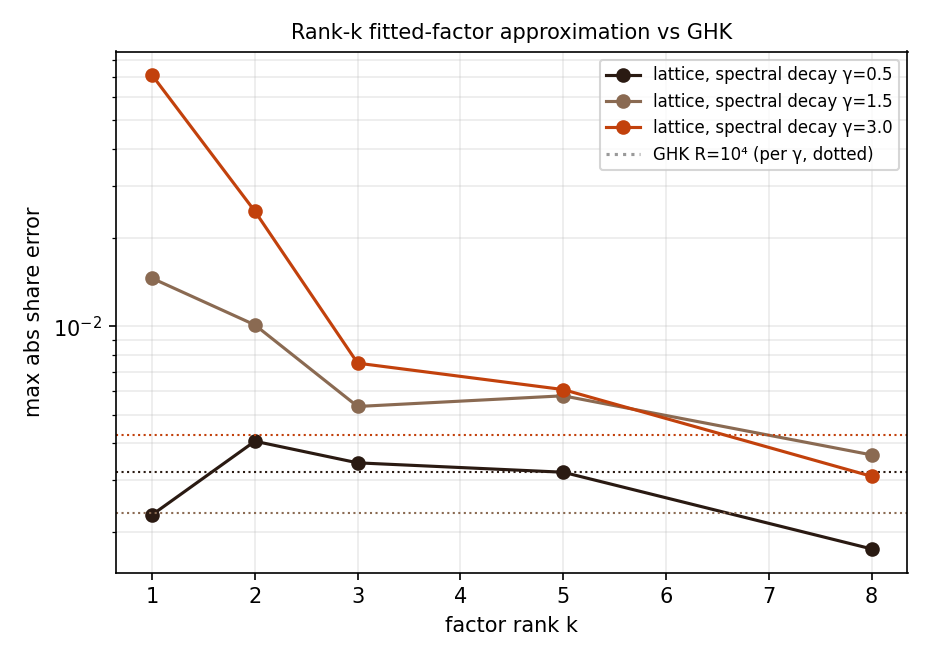
\includegraphics[width=0.66\textwidth]{figs/full_sigma.png}\\[4pt]
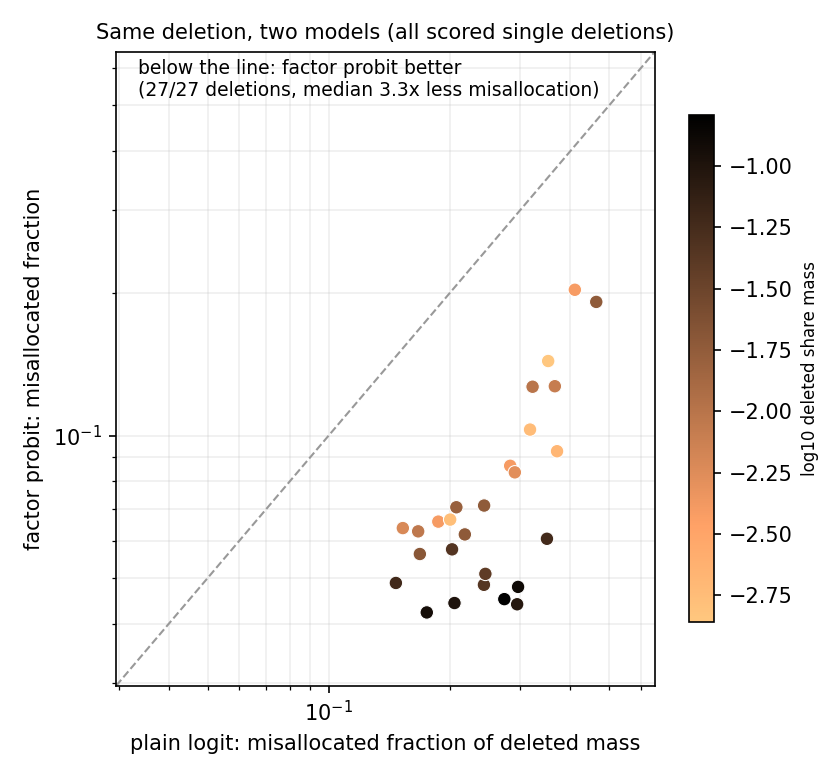
\includegraphics[width=0.66\textwidth]{figs/factorial.png}
\caption{Top: rank-$k$ contrast-space approximation error under spectral
decay $\gamma$ (dotted: GHK at $R=10^4$, per $\gamma$; not wall-time
matched). Bottom: paired comparison on identical deletions---plain
logit's misallocated fraction (horizontal) against factor probit's
(vertical), one point per scored single deletion, shaded by deleted mass;
the dashed line is parity.}
\label{fig:boundary}
\end{figure}

\section{Discussion}\label{sec:discussion}

Returning to our main limitation of fixed factors, estimation is the natural next step. With the reduced coordinates of
Proposition~\ref{prop:ident}, gradients of an outer likelihood or generalized method of moments
(GMM) objective pass through the calibration fixed point by implicit
differentiation. So there is a route to differentiable probit demand estimation at large
$N$. 

Of course, estimating $(V, D)$ rather than supplying them raises the usual
identification cautions: scale normalization, factor rotation, and the fact
that only difference covariances are identified. Rank and order
conditions for identifying error-component structures are given by
\citet{walker2007}. This is left to future work. 

Separately, the pass itself can be accelerated further. Its two stages
are smooth-kernel sums whose matrices are numerically low-rank in our
prototype tests, and a
Chebyshev-separated evaluation (in the spirit of black-box fast multipole methods) reduces
each node's cost from $O(NL)$ to $O(r(N+L))$, converging quickly in
$r$ in those tests. A forward-map prototype is committed (experiment 20). Its systematic
error control and extension to the derivative and calibration passes are
developed in a companion paper.

Beyond the Gaussian family, the same machinery computes races with arbitrary
alternative-specific idiosyncratic densities. Factor probit is best
seen as one point in a two-parameter family, base law by factor rank,
and every member runs through the same shared-field pass at the same
cost. Zero factors recovers the original transform. A common-scale
Gumbel base with zero loadings reproduces the Luce model exactly
\citep{luce1959,yellott1977}, and Gumbel with factors yields
correlated softmax.

Neither method class dominates the other. Simulation owns arbitrary
$\Sigma$ and coarse accuracy whereas the shared field owns the factor form,
tight accuracy, derivatives, and calibration. Our experiments give some guidance as to the boundary. 

In particular, covariance approximation rather than quadrature
becomes the binding limitation when the choice-relevant covariance is
not well represented at modest rank. We leave to future work a
walk-forward calibration on real assortment data. The empirical
accuracy evidence for probit against logit families is surveyed in
companion work \citep{cottonsurvey}.

\section{Potential applications}\label{sec:applications}

The territory is larger than econometrics. That is because a probit model is a race in which performances
are Gaussian, sometimes correlated. Races take many forms at all levels of spatial and temporal resolution. Predicting item selection and user clicks drives digital commerce, just as 
predicting market share is fundamental to company analysis. Countless choices are made by man, nature, and machine. Across all the world's applications
of large language models, perhaps a billion next-token choices are made a second.

Nature repeatedly poses the same computational problem: out of thousands, millions, or vastly more correlated alternatives---candidate crystal-growth directions, microscopic slip systems, adsorption geometries, pore-scale flow routes, turbulent modes, lightning leaders, fault asperities, or phase-transition seeds---which one wins first?

Materials science is especially rich in such races. Any one of a
thousand grain boundaries is a competitor at which fracture, diffusion,
segregation, or corrosion can initiate first. The same structure
appears in precipitation nuclei during alloy aging, hydrogen-trapping
sites in embrittlement, electrochemical reaction sites on an electrode,
dendrite formation in a battery, charge trapping in semiconductors, and
breakdown paths through a dielectric. Biology stages the same contest
among mutations and microbial lineages.

Astronomy alone offers several concrete instances. Which of many
catalog candidates is the true cross-match, which sky tile hosts a
gravitational-wave counterpart, which of a million nightly survey
alerts deserves follow-up. Each is a race among thousands of
alternatives whose scores share a few instrument and observing-condition
factors, and observing a candidate then re-ranking the rest is
precisely the removal counterfactual computed here.

It is not only horses that race. However, horse races are worthy of mention, and not only as regards attribution of a core trick used herein. For at least half a century those betting on them have been confronted by the nuances of choice and permutation probabilities in exacta, quinella, trifecta, and place betting. In that setting there has been a strong Darwinian selection that weeds out those anchoring to a simple renormalization of probability---this does not model second-place probabilities well at all if the favorite does not win \citep{henery1981,lo1994}.\footnote{The
Darwinian winner is instructive. \citet{benter1994}, whose Hong Kong
betting operations by his own concession made close to a billion
dollars overall \citep{chellel2018}, wrote of the simple
renormalization (the Harville formula) that it ``is significantly
biased, and should not be used for betting purposes.'' His fix
tempered the win probabilities before conditioning.}

At the racetrack both nature and the market make choices---the latter in risk-neutral probability. We do not always personify markets as choosers with revealed preferences but perhaps we should. 
Trillions of dollars are invested passively in capital-weighted indexes in a subtle, unwitting nod to that same simple renormalization deemed unworthy for the racetrack.

Why all this probit work? For anyone modeling performance directly,
Gaussian is the natural noise. Sums of many small effects are Gaussian,
and nobody measuring times, scores, or energies would posit
Gumbel-distributed performance. The Gumbel race is chosen backwards,
for the convenience of its winner probabilities. That convenience is
starkest when an item is removed from a list whose probabilities have
already been assigned.

The reflexive move is the renormalization already met at the
racetrack, dividing each survivor by the sum. It
feels like no assumption at all, and it is exactly the assumption that
performances are independent Gumbel draws. It is also built into the
output layer of most neural networks. The honest alternative,
recomputing the race under Gaussian performances, has been
understandably rare when the race involves a thousand competing choices
of token, crystal lattice point, or segment of the sky.

However we hope the main message is not lost. For fifty years, computability has been a very heavy factor in deciding which choice models get used. For
the factor form of probit, the form in which correlated utilities entered
econometrics \citep{hausman1978}, that constraint is in large part removed by our work. All shares, Jacobian--vector products, and
the inverse map remain comfortably below a minute at ten thousand alternatives and
rank two on the reported hardware. Integrating
factor estimation with this inner solver is, again, outside the present paper,
but with $(V, D)$ in hand at modest rank, the choice between logit and
factor probit becomes one of fit, not tractability.

\appendix
\section{Proof of Proposition~\ref{thm:inv}}\label{app:inv}

We show in order that the Jacobian $J = \partial p/\partial\mu$ is the
weighted graph Laplacian with weights $w_{ij}$ (Steps~1--4), that $J$ is
positive semidefinite with null space $\mathrm{span}\{\mathbf{1}\}$
(Step~5), and that $p$ restricted to $\mathbf{1}^\perp$ is a smooth
bijection onto the interior of the simplex (Steps~6--8). Throughout we
work in max-wins coordinates, condition on the factor draw $f$, write
$m_i(f) = \mu_i + v_i^\top f$ and let $g_i, F_i$ be the conditional
Gaussian density and CDF, so that
\[
p_i \;=\; \E_f \int g_i(x\mid f)\prod_{j\ne i} F_j(x\mid f)\,dx .
\]

\paragraph{Step 1: off-diagonal entries.} Fix $i\ne j$. The mean $\mu_j$
enters $p_i$ only through the single factor
$F_j(x\mid f) = \Phi\big((x - m_j(f))/\sqrt{D_j}\big)$, whose derivative is
\[
\frac{\partial}{\partial \mu_j} F_j(x\mid f) \;=\; -\,g_j(x\mid f).
\]
Differentiation under the integral and the expectation is legitimate
because the differentiated integrand is dominated, uniformly in
$(f,\mu)$, by an integrable bound:
\[
\int g_i(x\mid f)\, g_j(x\mid f)\,dx
\;=\; \frac{\exp\!\big[-(m_i(f)-m_j(f))^2 / (2(D_i+D_j))\big]}
{\sqrt{2\pi(D_i+D_j)}}
\;\le\; \frac{1}{\sqrt{2\pi(D_i+D_j)}} ,
\]
the equality being the Gaussian product integral and the inequality
bounding the exponential by one. Hence
\[
J_{ij} \;=\; \frac{\partial p_i}{\partial \mu_j}
\;=\; \E_f \int g_i \Big(\tfrac{\partial}{\partial\mu_j}F_j\Big)
\prod_{\ell\ne i,j}F_\ell\,dx
\;=\; -\,\E_f \int g_i\, g_j \prod_{\ell\ne i,j} F_\ell\,dx
\;=\; -\,w_{ij}.
\]

\paragraph{Step 2: symmetry.} The integrand
$g_i\, g_j \prod_{\ell\ne i,j}F_\ell$ is unchanged when $i$ and $j$ are
exchanged, so $w_{ij}=w_{ji}$ and $J_{ij}=J_{ji}$.

\paragraph{Step 3: diagonal entries.} Translation invariance
$p(\mu+c\mathbf{1})=p(\mu)$ (Proposition~\ref{prop:ident}) makes every
row of $J$ sum to zero, $J\mathbf{1}=0$, so
\[
J_{ii} \;=\; -\sum_{j\ne i} J_{ij} \;=\; \sum_{j\ne i} w_{ij}.
\]
The same value follows directly. Since
$\partial_{\mu_i} g_i(x\mid f) = -g_i'(x\mid f)$, integration by parts gives
\[
\frac{\partial p_i}{\partial \mu_i}
\;=\; \E_f \int (-g_i')\prod_{j\ne i}F_j\,dx
\;=\; \E_f \int g_i \sum_{j\ne i} g_j \prod_{\ell\ne i,j}F_\ell\,dx
\;=\; \sum_{j\ne i} w_{ij},
\]
the boundary terms vanishing because $g_i\to 0$ at $\pm\infty$ while
$\prod_{j\ne i}F_j$ stays bounded.

\paragraph{Step 4: the Laplacian form.} Each rank-one term
$w_{ij}(e_i-e_j)(e_i-e_j)^\top$ adds $+w_{ij}$ to the diagonal entries
$(i,i)$ and $(j,j)$ and $-w_{ij}$ to the off-diagonal entries $(i,j)$ and
$(j,i)$. Summing over unordered pairs reproduces exactly the entries of
Steps~1 and~3, so
\[
J \;=\; \sum_{i<j} w_{ij}(e_i-e_j)(e_i-e_j)^\top,
\qquad
h^\top J h \;=\; \sum_{i<j} w_{ij}\,(h_i-h_j)^2 ,
\]
the quadratic form following from $h^\top(e_i-e_j) = h_i-h_j$.

\paragraph{Step 5: positive definiteness on the quotient.} For every $f$
and finite $x$ the densities $g_i, g_j$ are strictly positive and each
$F_\ell(x\mid f)\in(0,1)$, so the integrand of $w_{ij}$ is strictly
positive and $w_{ij}>0$. The form
$h^\top J h = \sum_{i<j} w_{ij}(h_i-h_j)^2 \ge 0$ then vanishes only when
$h_i=h_j$ for every pair, i.e.\ when $h$ is constant. Thus $J$ is
symmetric positive semidefinite with null space exactly
$\mathrm{span}\{\mathbf{1}\}$, and $B^\top J B \succ 0$ for every
full-rank basis $B$ of $\mathbf{1}^\perp$. The identity $p=\nabla G$ for
$G(\mu)=\E\max_i\{\mu_i+\xi_i\}$ is the Williams--Daly--Zachary/McFadden
identity \citep{williams1977,daly1978,mcfadden1981}, so $J=\nabla^2 G$ is
the Hessian of the convex $G$.

\paragraph{Step 6: existence of the inverse.} Fix a strictly positive
target $\hat p$ in the interior of the simplex and minimize
\[
H(\mu) \;=\; G(\mu) - \hat p^\top \mu
\qquad \text{over } \mu\in\mathbf{1}^\perp .
\]
On $\mathbf{1}^\perp$, $H$ is strictly convex, its Hessian being the
reduced $J\succ0$ of Step~5. Since the shocks are centered, Jensen's
inequality gives
$G(\mu)=\E\max_i(\mu_i+\xi_i) \ge \max_i(\mu_i+\E\xi_i) = \max_i\mu_i$.
Using $\mathbf{1}^\top\hat p = 1$,
\begin{align*}
H(\mu)
&\;\ge\; \max_i \mu_i - \hat p^\top\mu
\;=\; \sum_i \hat p_i\big(\max_j \mu_j - \mu_i\big) \\
&\;\ge\; \hat p_{\min}\sum_i\big(\max_j\mu_j - \mu_i\big)
\;\ge\; \hat p_{\min}\big(\max_i\mu_i - \min_i\mu_i\big) \\
&\;\ge\; \hat p_{\min}\,\|\mu\|_\infty
\;\ge\; \hat p_{\min}\,\|\mu\|_2/\sqrt{N} .
\end{align*}
The second line uses $\hat p_i\ge \hat p_{\min}>0$ and
$\max_j\mu_j-\mu_i\ge 0$; the third keeps only the single term
$i=\arg\min_i\mu_i$; and the fourth uses that a mean-zero vector has
$\max_i\mu_i\ge 0\ge\min_i\mu_i$, so its range dominates
$\|\mu\|_\infty$. Hence $H(\mu)\to+\infty$ as $\|\mu\|_2\to\infty$ on
$\mathbf{1}^\perp$: $H$ is coercive and attains its minimum.

\paragraph{Step 7: the minimizer inverts $p$.} Because $D_i>0$, the
utilities have a smooth full-support joint density and ties are null, so
$\nabla G = p$. At the minimizer $\mu^\star$ the gradient of $H$ vanishes
on the constraint subspace, $B^\top(p(\mu^\star)-\hat p)=0$, so
$p(\mu^\star)-\hat p\in\mathrm{span}\{\mathbf{1}\}$. Both $p(\mu^\star)$
and $\hat p$ sum to one, so the constant is zero and $p(\mu^\star)=\hat
p$. Strict convexity makes $\mu^\star$ the unique mean-zero solution.

\paragraph{Step 8: smoothness.} The map $p$ is smooth and its reduced
Jacobian $B^\top J B$ is nonsingular everywhere on $\mathbf{1}^\perp$
(Step~5), so the inverse-function theorem makes $\hat p\mapsto
\mu^\star(\hat p)$ smooth on the interior of the simplex. This completes
the proof of Proposition~\ref{thm:inv}.

\section{Derivation of the conjugate trace identity}\label{app:trace}

Work in max-wins coordinates at fixed mean-zero $\mu$, with $\xi \sim
N(0, \Sigma)$, density $\varphi$, winner $I = \arg\max_i (\mu_i +
\xi_i)$, and choice cells $A_i = \{x : \mu_i + x_i \ge \mu_j + x_j
\ \forall j\}$.

\paragraph{Step 1: reduce to the winner's mean shock.} $G(\mu) =
\E[\mu_I + \xi_I] = \mu^\top p + \E[\xi_I]$, so the claim is
$\E[\xi_I] = \mathrm{tr}(\Sigma J)$.

\paragraph{Step 2: integrate by parts on each cell.} Since
$\nabla \varphi(x) = -\Sigma^{-1} x\, \varphi(x)$, we have $x
\varphi(x) = -\Sigma \nabla\varphi(x)$, and the divergence theorem
applied coordinatewise on the cell (Gaussian decay kills the boundary
at infinity) gives
\[
\E[\xi\, \mathbf{1}\{\xi \in A_i\}]
= \int_{A_i} x \varphi(x)\,dx
= -\Sigma \oint_{\partial A_i} \varphi(x)\, n(x)\, dS(x),
\]
with $n$ the outward unit normal and $dS$ surface measure.

\paragraph{Step 3: identify facet masses with photo-finish weights.}
The boundary of $A_i$ is the union of facets $F_{ij} = \{x : \mu_i +
x_i = \mu_j + x_j \ge \mu_\ell + x_\ell \ \forall \ell\}$ with
outward normal $n = (e_j - e_i)/\sqrt2$. The facet mass is the
photo-finish weight, $w_{ij} = \tfrac{1}{\sqrt2}\int_{F_{ij}}
\varphi\, dS$, the surface form of the weights of
Proposition~\ref{thm:inv} stated in the transport discussion. Hence
\[
\oint_{\partial A_i} \varphi\, n\, dS
= \sum_{j \ne i} \frac{e_j - e_i}{\sqrt2} \int_{F_{ij}} \varphi\, dS
= \sum_{j\ne i} (e_j - e_i)\, w_{ij},
\]
and therefore $\E[\xi\, \mathbf{1}\{I = i\}] = \Sigma \sum_{j \ne
i} w_{ij} (e_i - e_j)$. Its $i$th coordinate is $(\Sigma J)_{ii}$,
since $J e_i = \sum_{j \ne i} w_{ij}(e_i - e_j)$.

\paragraph{Step 4: sum over cells.} Using $w_{ij} = w_{ji}$ and
symmetrizing,
\[
\E[\xi_I] = \sum_i e_i^\top \Sigma \sum_{j\ne i} w_{ij}(e_i - e_j)
= \sum_{i<j} w_{ij}\, (e_i - e_j)^\top \Sigma\, (e_i - e_j)
= \mathrm{tr}(\Sigma J),
\]
and $(e_i - e_j)^\top \Sigma (e_i - e_j) = D_i + D_j + \|v_i -
v_j\|^2 = s_{ij}^2$. Finally $\Omega(p) = p^\top \mu - G(\mu) =
-\mathrm{tr}(\Sigma J)$ at $p = p(\mu)$. Experiment 27 verifies the
per-class identity $\E[\xi_i \mathbf{1}\{I=i\}] = (\Sigma J)_{ii}$
within Monte Carlo noise, the full identity to $3\times10^{-9}$, and
the binary closed form $\Omega = -s\,\phi(\Phi^{-1}(q))$ to
$3\times10^{-13}$.

\section*{Reproducibility and Supplementary Materials}
\sloppy

\begin{description}
\item[Code and experiments:] all numbers come from committed, seeded
scripts with correctness anchors run before any comparison (repository
experiments 13--27, 29--31, and 33--38, under
\texttt{research/experiments/}; experiment 28, which supports the
companion paper, and exploratory experiment 32 remain in the
\texttt{kinetics} research repository). A single manifest,
\texttt{research/experiments/run\_all\_paper.py}, regenerates every
table and figure; this paper is built from release \texttt{v1.1.0}
of the repository at \url{https://github.com/microprediction/winning},
whose package is on PyPI (\texttt{pip install winning}).
\item[Software:] the algorithm ships in the open-source
\texttt{winning} package \citep{winningpkg}, module
\texttt{winning.factor}, with an optional compiled Rust kernel
(\texttt{fastrace}); package--benchmark agreement is itself a reported
number.
\item[Data:] all experiments use synthetic data generated by the seeded
scripts; no external data are required.
\end{description}

Hardware and software: Apple M4, 16\,GB, Python 3.12.9,
NumPy 2.4.6, SciPy 1.18.0; compiled timings use rustc 1.97.1
(release profile, rayon defaulting to all performance cores); experiment 17 enforces single-threaded BLAS via
\texttt{threadpoolctl}; sub-second timings are warmed medians of three
runs, and long simulations are single realizations, disclosed as such.
Monte Carlo chunk sizes derive from an explicit 1.5\,GB memory budget, and
peak resident memory stays below 2\,GB.

\section*{Disclosure Statement}

The author reports no conflicts of interest. No external funding was
received for this work.

\begin{thebibliography}{9}
\bibitem[Aalen and Johansen(1978)]{aalen1978} O.~O. Aalen, S.~Johansen.
An empirical transition matrix for non-homogeneous Markov chains based on
censored observations. \emph{Scandinavian Journal of Statistics} 5
(1978) 141--150.

\bibitem[Albert and Chib(1993)]{albertchib1993} J.~H. Albert, S.~Chib.
Bayesian analysis of binary and polychotomous response data.
\emph{Journal of the American Statistical Association} 88 (1993)
669--679.

\bibitem[Ali(1998)]{ali1998} M.~M. Ali. Probability models on horse-race
outcomes. \emph{Journal of Applied Statistics} 25 (1998) 221--229.

\bibitem[Aurenhammer et~al.(1998)Aurenhammer, Hoffmann, and
Aronov]{aurenhammer1998} F.~Aurenhammer, F.~Hoffmann, B.~Aronov.
Minkowski-type theorems and least-squares clustering.
\emph{Algorithmica} 20 (1998) 61--76.

\bibitem[Bechhofer(1954)]{bechhofer1954} R.~E. Bechhofer. A single-sample
multiple decision procedure for ranking means of normal populations with
known variances. \emph{Annals of Mathematical Statistics} 25 (1954)
16--39.

\bibitem[Benter(1994)]{benter1994} W.~Benter. Computer based horse
race handicapping and wagering systems: a report. In D.~B. Hausch,
V.~S.~Y. Lo, W.~T. Ziemba (eds.), \emph{Efficiency of Racetrack
Betting Markets}, Academic Press, 1994, 183--198.

\bibitem[Berry(1994)]{berry1994} S.~Berry. Estimating discrete-choice
models of product differentiation. \emph{RAND Journal of Economics} 25
(1994) 242--262.

\bibitem[Berry et~al.(2013)Berry, Gandhi, and Haile]{bgh2013} S.~Berry, A.~Gandhi, P.~Haile. Connected substitutes
and invertibility of demand. \emph{Econometrica} 81 (2013) 2087--2111.

\bibitem[Berry et~al.(1995)Berry, Levinsohn, and Pakes]{berry1995} S.~Berry, J.~Levinsohn, A.~Pakes. Automobile prices in
market equilibrium. \emph{Econometrica} 63 (1995) 841--890.

\bibitem[Berthet et~al.(2020)Berthet, Blondel, Teboul, Cuturi, Vert, and
Bach]{berthet2020} Q.~Berthet, M.~Blondel, O.~Teboul, M.~Cuturi,
J.-P.~Vert, F.~Bach. Learning with differentiable perturbed optimizers. In
\emph{Advances in Neural Information Processing Systems} 33 (2020)
9508--9519.

\bibitem[Bhat(2011)]{bhat2011} C.~Bhat. The maximum approximate composite marginal
likelihood (MACML) estimation of multinomial probit-based unordered response
choice models. \emph{Transportation Research Part B} 45 (2011) 923--939.

\bibitem[Bliss(1934)]{bliss1934} C.~I. Bliss. The method of probits.
\emph{Science} 79 (1934) 38--39.

\bibitem[Bolduc(1999)]{bolduc1999} D.~Bolduc. A practical technique to
estimate multinomial probit models in transportation. \emph{Transportation
Research Part B} 33 (1999) 63--79.

\bibitem[Bonnet et~al.(2022)Bonnet, Galichon, Hsieh, O'Hara, and
Shum]{bonnet2022} O.~Bonnet, A.~Galichon, Y.-W. Hsieh, K.~O'Hara,
M.~Shum. Yogurts choose consumers? Estimation of random-utility models
via two-sided matching. \emph{Review of Economic Studies} 89 (2022)
3085--3114.

\bibitem[Botev(2017)]{botev2017} Z.~Botev. The normal law under linear restrictions:
simulation and estimation via minimax tilting. \emph{Journal of the
Royal Statistical Society B} 79 (2017)
125--148.

\bibitem[Butler and Moffitt(1982)]{butler1982} J.~S. Butler, R.~Moffitt. A computationally efficient
quadrature procedure for the one-factor multinomial probit model.
\emph{Econometrica} 50 (1982) 761--764.

\bibitem[Cao et~al.(2021)Cao, Genton, Keyes, and Turkiyyah]{cao2021} J.~Cao, M.~G. Genton, D.~E. Keyes, G.~M. Turkiyyah.
Exploiting low-rank covariance structures for computing high-dimensional
normal and Student-$t$ probabilities. \emph{Statistics and Computing} 31
(2021) 2.

\bibitem[Cao and Katzfuss(2026)]{cao2025} J.~Cao, M.~Katzfuss.
Linear-cost Vecchia approximation of multivariate normal probabilities.
\emph{Journal of the American Statistical Association} 121 (2026)
768--781.

\bibitem[Chang et~al.(2026)Chang, Narita, and Saito]{chang2022}
H.~Chang, Y.~Narita, K.~Saito. Approximating choice data by discrete
choice models. Working paper, arXiv:2205.01882, 2026 revision.

\bibitem[Chellel(2018)]{chellel2018} K.~Chellel. The gambler who
cracked the horse-racing code. \emph{Bloomberg Businessweek}, May 3,
2018.

\bibitem[Chia(2021)]{chia2021} A.~Chia. Automatically differentiable random coefficient
logistic demand estimation. arXiv:2106.04636 (2021).

\bibitem[Chiong et~al.(2016)Chiong, Galichon, and Shum]{chiong2016} K.~Chiong, A.~Galichon, M.~Shum. Duality in dynamic
discrete-choice models. \emph{Quantitative Economics} 7 (2016) 83--115.

\bibitem[Cohen(2010)]{cohen2010} M.~Cohen. A structured covariance
probit demand model. Food Marketing Policy Center Research Report 123,
University of Connecticut, 2010.

\bibitem[Collier et~al.(2021)Collier, Mustafa, Kokiopoulou, Jenatton,
and Berent]{collier2021} M.~Collier, B.~Mustafa, E.~Kokiopoulou,
R.~Jenatton, J.~Berent. Correlated input-dependent label noise in
large-scale image classification. \emph{Proceedings of the IEEE/CVF Conference on Computer Vision and
Pattern Recognition (CVPR)} (2021)
1551--1560.

\bibitem[Conlon and Gortmaker(2020)]{conlon2020} C.~Conlon, J.~Gortmaker. Best practices for
differentiated products demand estimation with PyBLP. \emph{RAND Journal of
Economics} 51 (2020) 1108--1161.

\bibitem[Connors et~al.(2014)Connors, Hess, and Daly]{connors2014} R.~Connors, S.~Hess, A.~Daly. Analytic approximations
for computing probit choice probabilities. \emph{Transportmetrica A} 10
(2014) 119--139.

\bibitem[Cotton(2021a)]{cotton2021} P.~Cotton. Inferring relative ability from winning
probability in multientrant contests. \emph{SIAM Journal on Financial Mathematics}
12 (2021) 295--317.

\bibitem[Cotton(2021b)]{winningpkg} P.~Cotton. The \texttt{winning} package: inference for multi-entrant contests,
2021. \url{https://github.com/microprediction/winning}.

\bibitem[Cotton(2026)]{cottonsurvey} P.~Cotton. Probit versus logit:
a survey of empirical accuracy. SSRN working paper, 2026.

\bibitem[Craig(2008)]{craig2008} P.~Craig. A new reconstruction of
multivariate normal orthant probabilities. \emph{Journal of the Royal
Statistical Society B} 70 (2008) 227--243.

\bibitem[Cunningham et~al.(2011)Cunningham, Hennig, and Lacoste-Julien]{cunningham2011} J.~P. Cunningham, P.~Hennig, S.~Lacoste-Julien.
Gaussian probabilities and expectation propagation. arXiv:1111.6832 (2011).

\bibitem[Curnow and Dunnett(1962)]{curnow1962} R.~N. Curnow, C.~W.
Dunnett. The numerical evaluation of certain multivariate normal
integrals. \emph{Annals of Mathematical Statistics} 33 (1962) 571--579.

\bibitem[Daganzo(1979)]{daganzo1979} C.~F. Daganzo. \emph{Multinomial
Probit: The Theory and Its Application to Demand Forecasting}. Academic
Press, 1979.

\bibitem[Daganzo et~al.(1977)Daganzo, Bouthelier, and
Sheffi]{daganzo1977} C.~F. Daganzo, F.~Bouthelier, Y.~Sheffi.
Multinomial probit and qualitative choice: a computationally efficient
algorithm. \emph{Transportation Science} 11 (1977) 338--358.

\bibitem[Daly and Zachary(1978)]{daly1978} A.~Daly, S.~Zachary.
Improved multiple choice models. In D.~Hensher, M.~Dalvi (eds.),
\emph{Determinants of Travel Choice}, Saxon House, 1978.

\bibitem[Dempster and Lerner(1950)]{dempster1950} E.~R. Dempster,
I.~M. Lerner. Heritability of threshold characters. \emph{Genetics} 35
(1950) 212--236.

\bibitem[Ding et~al.(2024)Ding, Imbens, Qu, and Ye]{ding2024} P.~Ding,
G.~Imbens, Z.~Qu, Y.~Ye. Computationally efficient estimation of large
probit models. arXiv:2407.09371 (2024).

\bibitem[Dunnett(1989)]{dunnett1989} C.~W. Dunnett. Algorithm AS 251:
multivariate normal probability integrals with product correlation
structure. \emph{Applied Statistics} 38 (1989) 564--579.

\bibitem[Elrod and Keane(1995)]{elrod1995} T.~Elrod, M.~P. Keane. A factor-analytic probit model for
representing the market structure in panel data. \emph{Journal of Marketing
Research} 32 (1995) 1--16.

\bibitem[Falconer(1965)]{falconer1965} D.~S. Falconer. The inheritance
of liability to certain diseases, estimated from the incidence among
relatives. \emph{Annals of Human Genetics} 29 (1965) 51--76.

\bibitem[Fasano and Denti(2025)]{fasano2025} A.~Fasano, F.~Denti. Multivariate Gaussian
cumulative distribution functions as the marginal likelihood of their
dual Bayesian probit models. \emph{Biometrika} 112 (2025) asaf060.

\bibitem[Finney(1947)]{finney1947} D.~J. Finney. \emph{Probit
Analysis: A Statistical Treatment of the Sigmoid Response Curve}.
Cambridge University Press, 1947.

\bibitem[Fosgerau et~al.(2020)Fosgerau, Melo, de~Palma, and
Shum]{fosgerau2020} M.~Fosgerau, E.~Melo, A.~de~Palma, M.~Shum. Discrete
choice and rational inattention: a general equivalence result.
\emph{International Economic Review} 61 (2020) 1569--1589.

\bibitem[Genton et~al.(2018)Genton, Keyes, and Turkiyyah]{genton2018}
M.~G. Genton, D.~E. Keyes, G.~M. Turkiyyah. Hierarchical decompositions for
the computation of high-dimensional multivariate normal probabilities.
\emph{Journal of Computational and Graphical Statistics} 27 (2018)
268--277.

\bibitem[Genz(1992)]{genz1992} A.~Genz. Numerical computation of multivariate normal
probabilities. \emph{Journal of Computational and Graphical
Statistics} 1 (1992)
141--149.

\bibitem[Genz and Bretz(2009)]{genzbretz2009} A.~Genz, F.~Bretz.
\emph{Computation of Multivariate Normal and $t$ Probabilities}. Lecture
Notes in Statistics 195, Springer, 2009.

\bibitem[Geweke et~al.(1994)Geweke, Keane, and Runkle]{geweke1994} J.~Geweke, M.~Keane, D.~Runkle. Alternative computational
approaches to inference in the multinomial probit model. \emph{Review of
Economics and Statistics} 76 (1994) 609--632.

\bibitem[Girolami and Rogers(2006)]{girolami2006} M.~Girolami,
S.~Rogers. Variational Bayesian multinomial probit regression with
Gaussian process priors. \emph{Neural Computation} 18 (2006) 1790--1817.

\bibitem[Gordy(2003)]{gordy2003} M.~B. Gordy. A risk-factor model
foundation for ratings-based bank capital rules. \emph{Journal of
Financial Intermediation} 12 (2003) 199--232.

\bibitem[Green and Swets(1966)]{green1966} D.~M. Green, J.~A. Swets.
\emph{Signal Detection Theory and Psychophysics}. Wiley, 1966.

\bibitem[Gupta(1963)]{gupta1963} S.~S. Gupta. Probability integrals of
multivariate normal and multivariate $t$. \emph{Annals of Mathematical
Statistics} 34 (1963) 792--828.

\bibitem[Haaijer et~al.(1998)Haaijer, Wedel, Vriens, and
Wansbeek]{haaijer1998} R.~Haaijer, M.~Wedel, M.~Vriens, T.~Wansbeek.
Utility covariances and context effects in conjoint MNP models.
\emph{Marketing Science} 17 (1998) 236--252.

\bibitem[Hajivassiliou and McFadden(1998)]{hajivassiliou1998} V.~Hajivassiliou, D.~McFadden. The method of
simulated scores for the estimation of LDV models. \emph{Econometrica} 66
(1998) 863--896.

\bibitem[Hajivassiliou et~al.(1996)Hajivassiliou, McFadden, and
Ruud]{hmr1996} V.~Hajivassiliou, D.~McFadden, P.~Ruud. Simulation of
multivariate normal rectangle probabilities and their derivatives:
theoretical and computational results. \emph{Journal of Econometrics} 72
(1996) 85--134.

\bibitem[Hausman and Wise(1978)]{hausman1978} J.~A. Hausman, D.~A.
Wise. A conditional probit model for qualitative choice: discrete
decisions recognizing interdependence and heterogeneous preferences.
\emph{Econometrica} 46 (1978) 403--426.

\bibitem[Heiss and Winschel(2008)]{heiss2008} F.~Heiss, V.~Winschel.
Likelihood approximation by numerical integration on sparse grids.
\emph{Journal of Econometrics} 144 (2008) 62--80.

\bibitem[Henery(1981)]{henery1981} R.~J. Henery. Permutation
probabilities as models for horse races. \emph{Journal of the Royal
Statistical Society B} 43 (1981) 86--91.

\bibitem[Herbrich et~al.(2006)Herbrich, Minka, and
Graepel]{herbrich2006} R.~Herbrich, T.~Minka, T.~Graepel. TrueSkill: a
Bayesian skill rating system. In \emph{Advances in Neural Information
Processing Systems} 19 (2006) 569--576.

\bibitem[Hotz and Miller(1993)]{hotz1993} V.~J. Hotz, R.~A. Miller. Conditional choice
probabilities and the estimation of dynamic models. \emph{Review of
Economic Studies} 60 (1993) 497--529.

\bibitem[Huch and Keane(2026)]{huch2026} E.~Huch, M.~Keane. Amortized inference for correlated
discrete choice models via equivariant neural networks. arXiv:2603.24705
(2026).

\bibitem[Kamakura(1989)]{kamakura1989} W.~A. Kamakura. The estimation
of multinomial probit models: a new calibration algorithm.
\emph{Transportation Science} 23 (1989) 253--265.

\bibitem[Kim et~al.(2026)Kim, Kang, Kock, Bansal, and Sohn]{kim2026}
G.~Kim, Y.~Kang, L.~Kock, P.~Bansal, K.~Sohn. Scalable variational
inference for multinomial probit models under large choice sets and
sample sizes. \emph{Statistics and Computing} 36 (2026) 47.

\bibitem[Kitagawa et~al.(2019)Kitagawa, M\'erigot, and
Thibert]{kmt2019} J.~Kitagawa, Q.~M\'erigot, B.~Thibert. Convergence of
a Newton algorithm for semi-discrete optimal transport. \emph{Journal
of the European Mathematical Society} 21 (2019) 2603--2651.

\bibitem[Lazear and Rosen(1981)]{lazear1981} E.~P. Lazear, S.~Rosen.
Rank-order tournaments as optimum labor contracts. \emph{Journal of
Political Economy} 89 (1981) 841--864.

\bibitem[L\'evy(2015)]{levy2015} B.~L\'evy. A numerical algorithm for
$L_2$ semi-discrete optimal transport in 3D. \emph{ESAIM: Mathematical
Modelling and Numerical Analysis} 49 (2015) 1693--1715.

\bibitem[Lee(2000)]{lee2000} L.-F. Lee. A numerically stable quadrature
procedure for the one-factor random-component discrete choice model.
\emph{Journal of Econometrics} 95 (2000) 117--129.

\bibitem[Lo and Bacon-Shone(1994)]{lo1994} V.~S.~Y. Lo, J.~Bacon-Shone.
A comparison between two models for predicting ordering probabilities in
multiple-entry competitions. \emph{The Statistician} 43 (1994) 317--327.

\bibitem[Loaiza-Maya and Nibbering(2022)]{loaiza2022} R.~Loaiza-Maya, D.~Nibbering. Scalable Bayesian
estimation in the multinomial probit model. \emph{Journal of Business \&
Economic Statistics} 40 (2022) 1678--1690.

\bibitem[Loaiza-Maya and Nibbering(2023)]{loaiza2023} R.~Loaiza-Maya,
D.~Nibbering. Fast variational Bayes methods for multinomial probit
models. \emph{Journal of Business \& Economic Statistics} 41 (2023)
1352--1363.

\bibitem[Lord(1952)]{lord1952} F.~M. Lord. \emph{A Theory of Test
Scores}. Psychometric Monograph No.~7, Psychometric Society, 1952.

\bibitem[Luce(1959)]{luce1959} R.~D. Luce. \emph{Individual Choice
Behavior: A Theoretical Analysis}. Wiley, 1959.

\bibitem[Mahani and Sharabiani(2019)]{mahani2019} A.~S. Mahani,
M.~T.~A. Sharabiani. Bayesian, and non-Bayesian, cause-specific
competing-risk analysis for parametric and nonparametric survival
functions: the R package CFC. \emph{Journal of Statistical Software} 89
(2019) 1--29.

\bibitem[McFadden(1981)]{mcfadden1981} D.~McFadden. Econometric models of probabilistic
choice. In C.~Manski, D.~McFadden (eds.), \emph{Structural Analysis of
Discrete Data with Econometric Applications}, MIT Press, 1981.

\bibitem[McFadden(1984)]{mcfadden1984} D.~McFadden. Econometric
analysis of qualitative response models. In Z.~Griliches,
M.~Intriligator (eds.), \emph{Handbook of Econometrics}, vol.~II,
North-Holland, 1984, 1395--1457.

\bibitem[Melo(2025)]{melo2025} E.~Melo. Learning in random utility
models via online decision problems. \emph{International Journal of
Economic Theory} 21 (2025) 494--526.

\bibitem[Mendell and Elston(1974)]{mendell1974} N.~R. Mendell, R.~C. Elston. Multifactorial
qualitative traits: genetic analysis and prediction of recurrence risks.
\emph{Biometrics} 30 (1974) 41--57.

\bibitem[Mi et~al.(2009)Mi, Miwa, and Hothorn]{mi2009} X.~Mi, T.~Miwa,
T.~Hothorn. mvtnorm: new numerical algorithm for multivariate normal
probabilities. \emph{The R Journal} 1 (2009) 37--39.

\bibitem[Miwa et~al.(2003)Miwa, Hayter, and Kuriki]{miwa2003} T.~Miwa,
A.~J. Hayter, S.~Kuriki. The evaluation of general non-centred orthant
probabilities. \emph{Journal of the Royal Statistical Society B} 65
(2003) 223--234.

\bibitem[Mosteller(1951)]{mosteller1951} F.~Mosteller. Remarks on the
method of paired comparisons: I. The least squares solution assuming
equal standard deviations and equal correlations. \emph{Psychometrika}
16 (1951) 3--9.

\bibitem[Norets and Takahashi(2013)]{norets2013} A.~Norets, S.~Takahashi. On the surjectivity of the
mapping between utilities and choice probabilities. \emph{Quantitative
Economics} 4 (2013) 149--155.

\bibitem[Ridgway(2016)]{ridgway2016} J.~Ridgway. Computation of Gaussian orthant
probabilities in high dimension. \emph{Statistics and Computing} 26 (2016)
899--916.

\bibitem[Sheffi et~al.(1982)Sheffi, Hall, and Daganzo]{sheffi1982}
Y.~Sheffi, R.~Hall, C.~F. Daganzo. On the estimation of the multinomial
probit model. \emph{Transportation Research Part A} 16 (1982) 447--456.

\bibitem[Stein(1981)]{stein1981} C.~M. Stein. Estimation of the mean
of a multivariate normal distribution. \emph{Annals of Statistics} 9
(1981) 1135--1151.

\bibitem[Stern(1992)]{stern1992} S.~Stern. A method for smoothing
simulated moments of discrete probabilities in multinomial probit
models. \emph{Econometrica} 60 (1992) 943--952.

\bibitem[Ta\c{s}kesen et~al.(2023)Ta\c{s}kesen, Shafieezadeh-Abadeh,
and Kuhn]{taskesen2023} B.~Ta\c{s}kesen, S.~Shafieezadeh-Abadeh,
D.~Kuhn. Semi-discrete optimal transport: hardness, regularization and
numerical solution. \emph{Mathematical Programming} 199 (2023)
1033--1106.

\bibitem[Thurstone(1927)]{thurstone1927} L.~L. Thurstone. A law of comparative judgment.
\emph{Psychological Review} 34 (1927) 273--286.

\bibitem[Tinessa(2021)]{tinessa2021} F.~Tinessa. Closed-form random
utility models with mixture distributions of random utilities:
exploring finite mixtures of qGEV models. \emph{Transportation
Research Part B} 146 (2021) 262--288.

\bibitem[Tinessa et~al.(2020)Tinessa, Marzano, and Papola]{tinessa2020}
F.~Tinessa, V.~Marzano, A.~Papola. Mixing distributions of tastes with
a Combination of Nested Logit (CoNL) kernel: formulation and
performance analysis. \emph{Transportation Research Part B} 141 (2020)
1--23.

\bibitem[Train(1995)]{train1995} K.~E. Train. Simulation methods for
probit and related models based on convenient error partitioning.
Working Paper 95-237, Department of Economics, University of
California, Berkeley, 1995.

\bibitem[Train(2009)]{train2009} K.~Train. \emph{Discrete Choice Methods with Simulation},
2nd ed. Cambridge University Press, 2009.

\bibitem[Vasicek(2002)]{vasicek2002} O.~Vasicek. Loan portfolio value.
\emph{Risk}, December 2002, 160--162.

\bibitem[Walker et~al.(2007)Walker, Ben-Akiva, and Bolduc]{walker2007}
J.~L. Walker, M.~Ben-Akiva, D.~Bolduc. Identification of parameters in
normal error component logit-mixture (NECLM) models. \emph{Journal of
Applied Econometrics} 22 (2007) 1095--1125.

\bibitem[Williams(1977)]{williams1977} H.~C.~W.~L. Williams. On the
formation of travel demand models and economic evaluation measures of
user benefit. \emph{Environment and Planning A} 9 (1977) 285--344.

\bibitem[Yellott(1977)]{yellott1977} J.~I. Yellott, Jr. The
relationship between Luce's choice axiom, Thurstone's theory of
comparative judgment, and the double exponential distribution.
\emph{Journal of Mathematical Psychology} 15 (1977) 109--144.

\end{thebibliography}

\end{document}
